\documentclass[11pt]{article}
\usepackage{acl}

\usepackage{times}
\usepackage{latexsym}
\usepackage[T1]{fontenc}
\usepackage[utf8]{inputenc}
\usepackage{microtype}
\usepackage{inconsolata}

\usepackage{booktabs}
\usepackage{multirow}
\usepackage{array}
\usepackage{graphicx}
\usepackage{subcaption}
\usepackage{amsmath}
\usepackage{amssymb}
\usepackage{enumitem}
\usepackage{xspace}
\usepackage{float}
\usepackage{placeins}
\usepackage{hyperref}
\usepackage{cleveref}

\newcommand{\eg}{\textit{e.g.}\xspace}
\newcommand{\ie}{\textit{i.e.}\xspace}
\newcommand{\vs}{\textit{vs.}\xspace}
\newcommand{\sd}{\sigma}
\newcommand{\se}{\mathrm{SE}}
\newcommand{\mean}{\mu}
\newcommand{\corr}{\mathrm{corr}}
\newcommand{\cohen}{d}
\newcommand{\pval}{p}

\title{The Missing Trade-Off: How LLMs Lose Human-Like Personality Structure}

\author{Anonymous Authors}

\begin{document}

\maketitle

% ============================================================
\begin{abstract}
Human personality is defined by trade-offs: conscientious individuals tend to be more emotionally stable, extraverts more open to experience. In large language models, these trade-offs simply vanish. Across 33 models from 15 families (61 Likert items, 12 seeds each), we find that (1)~model families produce systematically different response profiles (median pairwise $d = 1.01$), yet all scores compress toward the Likert midpoint; (2)~the Conscientiousness--Neuroticism correlation, a robust negative trade-off in humans ($r = -0.30$), \textbf{reverses} to strongly positive in LLMs ($r = +0.76$, 95\% CI $[0.58, 0.88]$), robustly replicated across subgroups; and (3)~surface-level prompt changes produce significant score shifts, confirming that these measurements lack full measurement invariance.
These findings indicate that LLM psychometric scores capture prompt-dependent response styles shaped by training and alignment, not human-like personality constructs. We recommend treating such measurements as probes of model behavioral tendencies rather than claims about personality.
\end{abstract}

\begin{figure}[!htb]
    \centering
    
\includegraphics[width=\columnwidth,height=0.42\textheight,keepaspectratio]{figures/intro_figure_prompt.pdf}
    \caption{\textbf{Core concept.} Identical psychometric items elicit systematically different Likert-scale responses from different models. These model-specific response style signatures raise the question: do psychometric scores in LLMs reflect personality traits, or systematic response tendencies shaped by training and alignment?}
    \label{fig:concept}
\end{figure}

% ============================================================
\section{Introduction}
\label{sec:intro}

Human personality is defined by trade-offs.
Conscientious individuals tend to be more emotionally stable; extraverts are typically more open to experience \citep{mccrae1992five, soto2017bfi2}.
These inter-dimension correlations are not incidental; they reflect genuine motivational and emotional tensions that make human personality what it is.
A growing number of studies apply personality inventories to LLMs and interpret the resulting scores as evidence for model ``personality traits'' \citep{jiang2023personality, pan2024personality, serapio-garcia2025personality}.
But a basic question has been largely overlooked: \emph{do these scores reproduce the trade-offs that define human personality?}
If LLM psychometric responses lack the correlational structure of human traits, if conscientious and neurotic no longer trade off, then applying personality labels to LLMs is, at best, misleading.

We argue that LLM questionnaire responses are better understood as \textit{response styles}: systematic tendencies shaped by training data, alignment objectives, and deployment configurations, rather than genuine personality traits \citep{paulhus1991response, binz2023psychology}.
If this is correct, two testable predictions follow: (1)~different models should exhibit systematically different response patterns, and (2)~the inter-dimension correlation structure should diverge from the human baseline. In particular, the characteristic trade-offs should be absent.

Existing work provides suggestive but incomplete evidence on this point.
\citet{schaekermann2024personality} found moderate-to-large inter-model differences across 9 LLMs, and \citet{serapio-garcia2025personality} evaluated 18 models but with heterogeneous APIs and no structural validity testing.
\citet{salecha2024social} and \citet{dominguez-olmedo2024questioning} documented compressed response distributions, while \citet{braun2025acquiescence} found systematic acquiescence bias.
However, no study has tested whether the \emph{inter-dimension correlation structure} of LLM responses matches the human baseline, a necessary condition for claiming structural equivalence.

We address this gap with the largest cross-family comparison to date: 33 models from 15 families, 9 psychometric dimensions, 61 Likert items, 12 seeds per model, all administered via unified APIs (Figure~\ref{fig:concept}).
Our contributions are:

\begin{enumerate}[leftmargin=*,nosep]
    \item \textbf{The largest unified cross-family response style comparison.}
    15 model families under controlled API conditions reveal large, systematic behavioral differences (median pairwise Cohen's $d = 1.01$), establishing that training and alignment leave measurable fingerprints on model responses.

    \item \textbf{A structural validity test revealing a missing trade-off.}
    The Conscientiousness--Neuroticism correlation, a robust negative trade-off in humans ($r = -0.30$) \citep{soto2017bfi2}, \textbf{reverses to strongly positive} in LLMs ($r = +0.76$, 95\% CI $[0.58, 0.88]$, $p < 0.001$, $n = 33$).
    This reversal is individually significant, replicates across all subgroups, and constitutes the primary evidence that human personality trade-offs do not transfer to LLMs.

    \item \textbf{Direct evidence against trait interpretation.}
    Surface-level prompt changes produce modest but significant score shifts (prompt explains 1--9\% of variance vs.\ 10--78\% for model family), with some rank instability across framings, confirming that these measurements lack full measurement invariance.
\end{enumerate}

Together, these findings challenge the interpretation of LLM psychometric scores as personality traits: model families do exhibit different behavioral fingerprints, but the structural architecture that defines human personality, its characteristic trade-offs, is absent.

\begin{figure}[!htb]
    \centering
    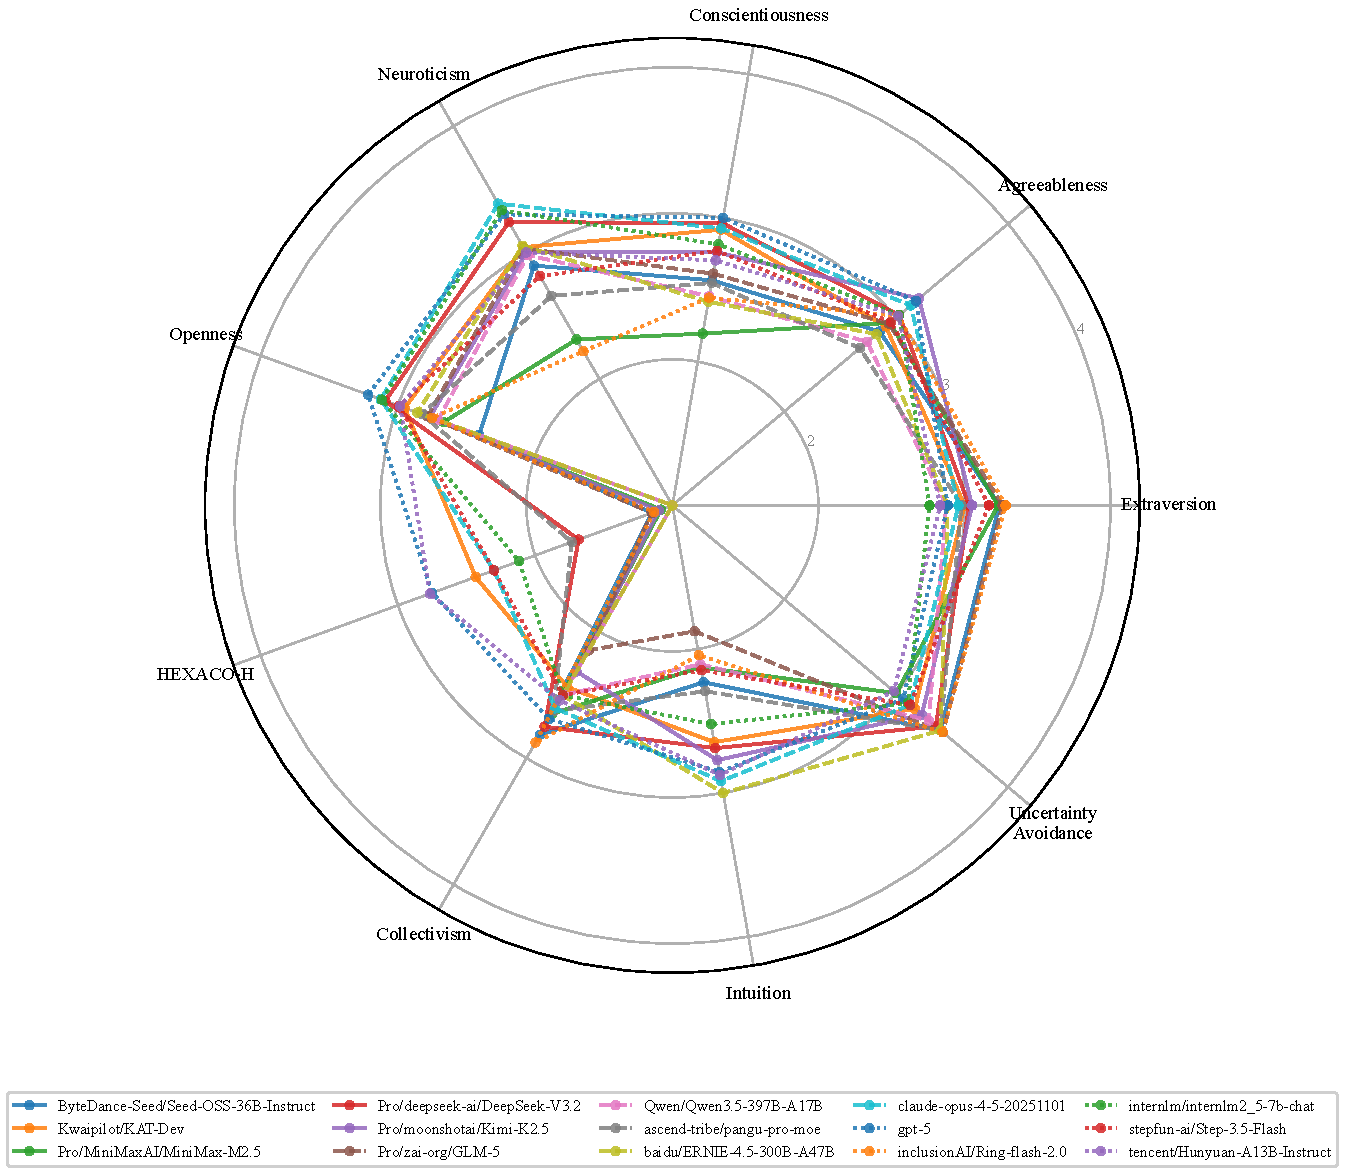
\includegraphics[width=0.48\textwidth]{figures/fig1_radar_combined.pdf}
    \caption{Response style profiles of all 15 model families across 9 dimensions. Each line is one model family. The distinct shapes suggest that different training approaches leave different behavioral fingerprints on models.}
    \label{fig:radar_profiles}
\end{figure}

\FloatBarrier

% ============================================================
\section{Related Work}
\label{sec:related}

\paragraph{LLM personality measurement.}
A growing body of work administers personality inventories to LLMs and interprets the resulting scores as trait profiles.
\citet{jiang2023personality} found temperature-dependent variation in ChatGPT using the BFI-10; \citet{pan2024personality} compared LLMs from different cultural backgrounds on the BFI-44; \citet{schaekermann2024personality} examined 9 LLMs on the Big Five, finding moderate-to-large inter-model differences.
\citet{serapio-garcia2025personality} proposed a psychometric framework for evaluating personality traits across 18 LLMs, the largest study to date, but with heterogeneous APIs and no structural validity testing.
\citet{hilliard2024eliciting} confirmed that model scale affects elicited profiles, and \citet{bodroza2024personality} found limited temporal stability but consistently elevated prosociality.
\citet{sorokovikova2024big} found systematic deviations from human norms, and \citet{tosato2025instability} documented persistent instability across scales and conversation histories.
These studies establish that LLMs produce variable, model-dependent psychometric profiles, but they do not test whether these profiles reproduce the \emph{inter-dimension correlation structure} that defines human personality, a necessary condition for claiming structural equivalence.

\paragraph{Trade-offs in human personality structure.}
The Five-Factor Model \citep{mccrae1992five} provides the theoretical foundation for the BFI dimensions we use.
A robust finding across large-scale validation studies is that personality dimensions exhibit systematic negative correlations: Conscientiousness--Neuroticism ($r = -0.30$), Extraversion--Neuroticism ($r = -0.34$), and Openness--Agreeableness ($r = +0.14$) \citep{soto2017bfi2}.
These trade-offs reflect genuine motivational and emotional tensions; conscientious individuals tend to be more emotionally stable, not because of measurement artifact, but because self-regulation and emotional reactivity are psychologically antagonistic.
If LLM psychometric scores correspond to human personality constructs, these trade-offs should be preserved.
\citet{suh2024rediscovering} recovered the Big Five factor structure from LLMs using semantic embeddings, but semantic structure and questionnaire response structure are distinct probes; we test the latter.
Our contribution is to directly test whether these human trade-offs survive in LLM questionnaire responses.

\paragraph{Measurement validity challenges.}
Applying human psychometric instruments to LLMs raises fundamental validity concerns \citep{schaekermann2024personality, serpell2024validity}.
\citet{suh2023challenging} question whether standard personality tests are valid for LLMs at all, given the lack of genuine self-report.
\citet{salecha2024social} demonstrated human-like social desirability biases; \citet{dominguez-olmedo2024questioning} showed compressed response distributions lacking natural variation; \citet{braun2025acquiescence} documented systematic acquiescence bias.
\citet{han2025personality} demonstrated a dissociation between LLM self-reported personality and behavioral choices.
\citet{xie2025aipsychobench} introduced AIPsychoBench, finding systematic discrepancies between LLM and human response patterns.
While prior work has raised validity concerns about individual biases, ours is the first to systematically document a \emph{structural reversal}, namely the disappearance of the Conscientiousness--Neuroticism trade-off, across a large sample of model families, and to demonstrate that these measurements lack prompt-invariance.

% ============================================================
\section{Method}
\label{sec:method}

\begin{figure*}[!t]
    \centering
    
\includegraphics[width=0.95\textwidth]{figures/framework_figure_prompt.pdf}
    \caption{\textbf{Experimental pipeline.} We select 15 model families via unified API platforms, query each model on 61 Likert items (9 dimensions, 12 seeds), collect 24,108 responses across 33 models, and apply a multi-module analysis framework (ANOVA, Cohen's $d$, convergent validity, reliability, acquiescence correction) to characterize model-level response style variation.}
    \label{fig:pipeline}
\end{figure*}

\subsection{Psychometric Instruments}
\label{sec:instruments}

We use 9 dimensions comprising 61 Likert items (1--5 scale; Table~\ref{tab:instruments}).
Five come from the Big Five Inventory \citep{john1999bigfive, mccrae1992five, soto2017bfi2}: Extraversion (8 items), Agreeableness (9), Conscientiousness (9), Neuroticism (8), and Openness (10).
We add HEXACO Honesty-Humility (5 items; \citealp{lee2004hexaco}), Collectivism (4 items; Schwartz Values Survey \citealp{schwartz1992universals}), Intuition (4 items; cognitive style), and Uncertainty Avoidance (4 items; cultural dimensions).
Reverse-scored items are transformed via $\text{score} = 6 - \text{original}$; dimension scores are the mean of constituent items.

\begin{table}[!htb]
\centering
\footnotesize
\caption{Psychometric instruments: 9 dimensions, 61 Likert items (1--5 scale).}
\label{tab:instruments}
\resizebox{\columnwidth}{!}{%
\begin{tabular}{llcc}
\toprule
Dimension & Source & Items & Reverse Scored \\
\midrule
Extraversion & BFI-44 & 8 & 4 items \\
Agreeableness & BFI-44 & 9 & 4 items \\
Conscientiousness & BFI-44 & 9 & 4 items \\
Neuroticism & BFI-44 & 8 & 2 items \\
Openness & BFI-44 & 10 & 3 items \\
HEXACO-H & HEXACO & 5 & 0 \\
Collectivism & Schwartz & 4 & 0 \\
Intuition & Cognitive Style & 4 & 2 items \\
Uncertainty Avoidance & Cultural Dimensions & 4 & 2 items \\
\midrule
\multicolumn{2}{l}{Total} & \textbf{61} & \\
\bottomrule
\end{tabular}%
}
\end{table}

\subsection{What We Measure: Response Style}
\label{sec:response_style}

We frame our measurements as \textbf{response style} rather than personality \citep{paulhus1991response, rammstedt2000response}.
In psychometrics, response style refers to systematic tendencies in how respondents answer questionnaire items, independent of item content: acquiescence (yea-saying), midpoint responding, extreme responding, and socially desirable responding \citep{baumgartner2007modeling}.
These styles are properties of the \emph{respondent}, not of the construct being measured.

Crucially, personality is not defined by individual dimension scores alone; it is defined by the \textbf{trade-offs between dimensions}.
The finding that conscientious individuals tend to be less neurotic ($r = -0.30$) \citep{soto2017bfi2} reflects a genuine psychological tension, not a measurement artifact.
If LLM psychometric scores do not reproduce these trade-offs, then the dimension labels (``Conscientiousness,'' ``Neuroticism'') do not denote the same constructs they denote in humans, regardless of how the individual scores distribute.

We adopt the response style framing because LLMs lack the subjective experience that personality constructs presume.
Our research question is therefore: \emph{do LLM responses reproduce the inter-dimension trade-offs that define human personality, or do they reflect prompt-dependent response styles?}
We explicitly test this by comparing LLM inter-dimension correlations against published human baselines (Section~\ref{sec:interdim}).

\subsection{Model Selection}
\label{sec:models}

We select 15 model families accessible through unified API platforms, contributing one representative model each (Table~\ref{tab:models}).
Priorities: flagship models where available; Dense and MoE architectures both represented (10 Dense, 5 MoE).

\begin{table}[!htb]
\centering
\footnotesize
\caption{Models from 15 model families, one representative model per family. Total parameters in parentheses where publicly disclosed.}
\label{tab:models}
\resizebox{\columnwidth}{!}{%
\begin{tabular}{lllc}
\toprule
\# & Model Family & Model ID & Architecture \\
\midrule
1 & Qwen & Qwen3.5-397B-A17B & MoE (397B) \\
2 & DeepSeek & DeepSeek-V3.2 & MoE (671B) \\
3 & GLM & GLM-5 & MoE (744B) \\
4 & Kimi & Kimi-K2.5 & MoE (1.1T) \\
5 & ERNIE & ERNIE-4.5-300B-A47B & MoE (300B) \\
6 & Hunyuan & Hunyuan-A13B-Instruct & Dense (13B) \\
7 & Seed & Seed-OSS-36B-Instruct & Dense (36B) \\
8 & InternLM & internlm2\_5-7b-chat & Dense (7B) \\
9 & Ring & Ring-flash-2.0 & MoE (100B) \\
10 & Step & Step-3.5-Flash & MoE (197B) \\
11 & Pangu & pangu-pro-moe & MoE (72B) \\
12 & KAT & KAT-Dev & Dense (32B) \\
13 & MiniMax & MiniMax-M2.5 & MoE (230B) \\
14 & GPT & GPT-5 & Undisclosed \\
15 & Claude & Claude Opus~4.5 & Undisclosed \\
\bottomrule
\end{tabular}%
}
\end{table}

\subsection{Experimental Protocol}
\label{sec:protocol}

Each model is administered all 61 items per seed at temperature $= 0.7$, with 12 seeds (0, 1, 2, 4, 5, 6, 7, 8, 9, 42, 123, 456) capturing response distribution variation, totaling 10,980 API calls.
We set temperature to 0.7 to balance response diversity with reproducibility. Temperature 0 yields deterministic outputs that eliminate within-model variance entirely, while higher temperatures ($\geq 1.0$) tend to produce inconsistent self-referential responses.
Prior work on LLM personality \citep{jiang2023personality} has shown that temperature affects reported trait scores, making a moderate temperature necessary to capture the full range of each model's response tendencies.
Items are framed as self-referential statements (\eg ``I see myself as someone who is the life of the party'') with a 1--5 agreement scale.
Rate limiting uses exponential backoff on 429 responses with up to 5 concurrent threads.

\subsection{Analysis Framework}
\label{sec:analysis}

Figure~\ref{fig:pipeline} illustrates the full experimental pipeline.
Our analysis combines several complementary approaches.
For each dimension, we run a one-way ANOVA (Model Family, 15 levels) with FDR-corrected $p$-values \citep{benjamini1995controlling} and partial $\eta^2_p$, supplemented by ordered logistic regression to account for the ordinal nature of Likert responses.
Pairwise Cohen's $d$ (Welch's $t$-test) is computed for all 105 model pairs across 8 primary dimensions (840 tests, FDR-corrected); power analysis confirms adequate power ($>80\%$) for $d \geq 0.8$ with 12 observations per model.
To correct for acquiescence bias, we compute partial correlations controlling for the first principal component (PC1).
We assess reliability via ICC(1,1) and coefficient of variation, classify dimensions with inter-model $\sd < 0.15$ as alignment artifacts, and compare LLM inter-dimension correlations against published human baselines \citep{john1999bigfive} for 5 key dimension pairs.
For all correlation and ANOVA analyses, we first aggregate the 12 seed-level responses per model into dimension means, then compute statistics at the model-family level ($n = 15$ for primary analyses; $n = 33$ for replication).
The human baseline correlations are drawn from large-scale BFI validation studies \citep{soto2017bfi2, vanderlinden2010general} and the trait taxonomy chapter \citep{john1999bigfive}; we report values from the Internet sample of \citet{soto2017bfi2} ($N = 1{,}000$).

% ============================================================
\section{Experiments}
\label{sec:results}

\FloatBarrier

\subsection{Overview}
\label{sec:overview}

Table~\ref{tab:model_means} reports model family mean scores across 9 dimensions.
On the Big Five, scores cluster around the scale midpoint (2.7--3.3) with the exception of Neuroticism, where Ring (2.22) and MiniMax (2.31) stand apart from GPT (3.30) and Claude (3.39).
Intuition shows the widest spread among non-H dimensions: GLM scores lowest (1.88) while Claude leads (2.92), a gap of over one full point.
Collectivism and Uncertainty Avoidance are the most compressed dimensions (ranges of 0.73 and 0.44, respectively), suggesting near-uniform responses across model families.
In the raw data, Dense models (GPT, Claude, Kimi, Hunyuan, Seed, InternLM, Ring, Step, KAT, MiniMax) tend to score higher on HEXACO-H and Agreeableness than MoE models, while MoE models show higher Uncertainty Avoidance. We revisit this pattern in Appendix~\ref{sec:appendix_hexaco_detail} with appropriate caution about confounding between architecture, provider, and scale.
Figure~\ref{fig:radar_profiles} overlays all 15 profiles, revealing that models from the same provider tend to share similar profile shapes.
Family-level clustering is further illustrated by within-family trajectories across model versions (Appendix~\ref{sec:appendix_trajectories}).

\begin{table*}[!t]
\centering
\caption{Model family mean scores (SD) across 9 dimensions. Range: 1--5. Primary analysis uses 8 dimensions ($\alpha > 0.70$); HEXACO-H ($\alpha = 0.27$) shown for completeness only.}
\label{tab:model_means}
\resizebox{\textwidth}{!}{%
\begin{tabular}{lccccccccc}
\toprule
Model Family & Extraversion & Agreeableness & Conscientiousness & Neuroticism & Openness & HEXACO-H & Collectivism & Intuition & UA \\
\midrule
ERNIE & 2.89 (0.14) & 2.82 (0.07) & 2.42 (0.10) & 3.05 (0.14) & 2.86 (0.14) & 1.00 (0.00) & 2.50 (0.21) & 3.00 (0.15) & 3.40 (0.20) \\
Seed & 3.24 (0.26) & 2.85 (0.27) & 2.56 (0.33) & 2.90 (0.25) & 2.41 (0.36) & 1.15 (0.15) & 2.81 (0.26) & 2.23 (0.39) & 3.40 (0.25) \\
DeepSeek & 3.03 (0.29) & 3.03 (0.23) & 2.96 (0.14) & 3.24 (0.24) & 3.09 (0.17) & 1.68 (0.34) & 2.75 (0.24) & 2.69 (0.19) & 3.35 (0.23) \\
Pangu & 2.98 (0.24) & 2.68 (0.21) & 2.55 (0.24) & 2.66 (0.29) & 2.82 (0.35) & 1.73 (0.37) & 2.62 (0.25) & 2.29 (0.28) & 3.40 (0.23) \\
InternLM & 2.76 (0.24) & 3.03 (0.14) & 2.81 (0.17) & 3.33 (0.19) & 3.12 (0.24) & 2.12 (0.38) & 2.50 (0.18) & 2.52 (0.23) & 3.10 (0.25) \\
KAT & 3.00 (0.00) & 2.91 (0.21) & 2.92 (0.14) & 3.04 (0.11) & 2.95 (0.14) & 2.43 (0.27) & 2.44 (0.19) & 2.65 (0.20) & 3.17 (0.16) \\
MiniMax & 3.23 (0.34) & 2.94 (0.25) & 2.19 (0.21) & 2.31 (0.22) & 2.67 (0.15) & 1.08 (0.23) & 2.65 (0.27) & 2.12 (0.13) & 3.00 (0.34) \\
Kimi & 3.05 (0.18) & 3.20 (0.12) & 2.76 (0.15) & 3.00 (0.11) & 2.77 (0.17) & 1.10 (0.13) & 2.31 (0.11) & 2.77 (0.31) & 3.23 (0.33) \\
Qwen & 2.88 (0.17) & 2.74 (0.26) & 2.45 (0.11) & 2.98 (0.17) & 2.71 (0.17) & 1.00 (0.00) & 2.50 (0.00) & 2.10 (0.17) & 3.29 (0.14) \\
Step & 3.17 (0.16) & 2.95 (0.16) & 2.77 (0.26) & 2.81 (0.26) & 2.99 (0.18) & 2.30 (0.64) & 2.50 (0.18) & 2.15 (0.61) & 3.12 (0.23) \\
Hunyuan & 2.83 (0.14) & 3.02 (0.09) & 2.70 (0.14) & 3.00 (0.00) & 2.98 (0.14) & 2.77 (0.27) & 2.54 (0.14) & 2.88 (0.13) & 2.98 (0.07) \\
GLM & 3.26 (0.26) & 2.94 (0.13) & 2.61 (0.24) & 3.03 (0.19) & 2.78 (0.19) & 1.15 (0.12) & 2.15 (0.13) & 1.88 (0.17) & 3.42 (0.16) \\
Ring & 3.28 (0.40) & 3.02 (0.36) & 2.44 (0.40) & 2.22 (0.29) & 2.75 (0.34) & 1.13 (0.26) & 2.88 (0.36) & 2.04 (0.46) & 3.42 (0.33) \\
GPT & 2.89 (0.17) & 3.18 (0.29) & 3.00 (0.17) & 3.30 (0.16) & 3.22 (0.37) & 2.75 (0.44) & 2.69 (0.30) & 2.85 (0.27) & 3.06 (0.26) \\
Claude & 2.96 (0.18) & 3.13 (0.18) & 2.93 (0.21) & 3.39 (0.19) & 3.12 (0.17) & 2.30 (0.32) & 2.60 (0.13) & 2.92 (0.12) & 3.12 (0.13) \\
\bottomrule
\end{tabular}%
}
\end{table*}

\subsection{Cross-Model Discrimination}
\label{sec:discrimination}

All 8 primary dimensions show significant model effects ($p < 0.001$, FDR-corrected; Table~\ref{tab:anova_results}), with the strongest discrimination on Neuroticism ($F = 34.60$, $\eta^2_p = 0.75$) and Intuition ($F = 20.26$, $\eta^2_p = 0.63$); non-parametric Kruskal-Wallis tests confirm these results.
Figure~\ref{fig:intermodel_sd} shows the inter-model $\sd$ by dimension: among the 8 primary dimensions, Intuition (0.37) and Neuroticism (0.34) show the most variability, while Agreeableness ($\sd = 0.15$) and UA ($\sd = 0.16$) fall below our alignment-artifact threshold of 0.15.
HEXACO-H has the highest overall variability (0.67) but is excluded from primary analysis ($\alpha = 0.27$); detailed results are in Appendix~\ref{sec:appendix_hexaco_detail}.

Architecture type (Dense vs.\ MoE) shows significant differences on several dimensions (Table~\ref{tab:architecture_effects}), with 10 Dense and 5 MoE families.
The strongest signals are on Agreeableness ($d = 0.78$, $p < 0.001$) and UA ($d = -0.83$, $p < 0.001$); HEXACO-H shows a larger apparent effect ($d = 0.91$) but is excluded from primary analysis due to low reliability ($\alpha = 0.27$).
\textbf{However, architecture is fully confounded with provider} (all MoE models are from a subset of providers, while Dense models include GPT and Claude) and partially confounded with model scale, so these patterns must be interpreted as descriptive observations of co-variation rather than evidence for causal architecture effects.

\begin{figure}[!htb]
    \centering
    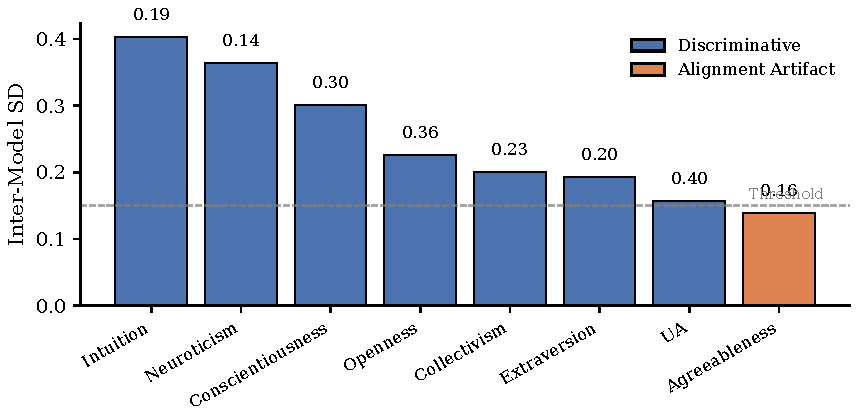
\includegraphics[width=0.48\textwidth]{figures/fig3_intermodel_sd.pdf}
    \caption{Inter-model SD by dimension. Blue: discriminative ($\sd \geq 0.15$); orange: alignment artifact. HEXACO-H ($\alpha = 0.27$) shown for completeness.}
    \label{fig:intermodel_sd}
\end{figure}

\begin{table}[!htb]
\centering
\caption{Mean dimension scores by architecture type (9 dimensions). Dense: $n = 10$ model families (GPT, Claude, Kimi, Hunyuan, Seed, InternLM, Ring, Step, KAT, MiniMax). MoE: $n = 5$ (Qwen, DeepSeek, GLM, ERNIE, Pangu). 95\% CI for Cohen's $d$ from bootstrap ($5{,}000$ iterations). Effects surviving FDR correction are marked with *; no claim of causal architecture effect is intended due to confounding with provider and scale. HEXACO-H ($\alpha = 0.27$) shown for completeness.}
\label{tab:architecture_effects}
\resizebox{\columnwidth}{!}{%
\footnotesize
\begin{tabular}{lcccc}
\toprule
Dimension & Dense & MoE & $d$ (95\% CI) & $p$ \\
\midrule
Extraversion         & 3.04 & 3.01 & +0.12 [$-$0.18, +0.42] & 0.42 \\
Agreeableness        & 3.02 & 2.84 & +0.78 [+0.47, +1.11] & 0.000* \\
Conscientiousness    & 2.71 & 2.60 & +0.36 [+0.07, +0.70] & 0.014 \\
Neuroticism          & 2.93 & 2.99 & $-$0.16 [$-$0.42, +0.12] & 0.25 \\
Openness             & 2.90 & 2.85 & +0.14 [$-$0.14, +0.43] & 0.32 \\
HEXACO-H             & 2.00 & 1.31 & +1.02 [+0.66, +1.20] & 0.000* \\
Collectivism         & 2.59 & 2.50 & +0.32 [+0.01, +0.64] & 0.046 \\
Intuition            & 2.51 & 2.39 & +0.27 [$-$0.03, +0.60] & 0.093 \\
UA                   & 3.16 & 3.37 & $-$0.83 [$-$1.15, $-$0.55] & 0.000* \\
\bottomrule
\end{tabular}%
}
\end{table}

\begin{table}[!htb]
\centering
\caption{ANOVA results: model effect on each dimension ($df = 14, 165$). Primary analysis uses 8 dimensions ($\alpha > 0.70$); HEXACO-H ($\alpha = 0.27$) shown for completeness. All $p < 0.001$ after FDR correction.}
\label{tab:anova_results}
\resizebox{\columnwidth}{!}{%
\footnotesize
\begin{tabular}{lrrrrr}
\toprule
Dimension & $F$ & $p$ (raw) & $\eta^2_p$ & KW $H$ & KW $p$ \\
\midrule
Extraversion         &   6.55 &  2.0e-10 &  0.357 &  65.5 &  1.3e-08 \\
Agreeableness        &   5.99 &  1.8e-09 &  0.337 &  62.4 &  4.4e-08 \\
Conscientiousness    &  14.35 &  4.8e-22 &  0.549 &  99.1 &  7.1e-15 \\
Neuroticism          &  34.60 &  8.1e-42 &  0.746 & 124.7 &  7.6e-20 \\
Openness             &   9.95 &  6.7e-16 &  0.458 &  80.2 &  2.6e-11 \\
\midrule
HEXACO-H             &  66.84 &  1.1e-16 &  0.851 & 163.7 &  4.5e-27 \\
Collectivism         &   9.01 &  1.9e-14 &  0.433 &  78.7 &  4.9e-11 \\
Intuition            &  20.26 &  5.5e-29 &  0.632 & 118.5 &  1.3e-18 \\
UA                   &   5.68 &  6.3e-09 &  0.325 & 62.3 & 4.6e-08 \\
\bottomrule
\end{tabular}%
}
\end{table}

The pairwise effect sizes are large: the median Cohen's $d$ across all 105 model pairs and 8 primary dimensions is 1.01, and every pair exceeds $d \geq 0.8$ on at least one dimension (Figure~\ref{fig:cohen_d_heatmap}).
Table~\ref{tab:top_cohen_d} reports the largest pairwise Cohen's $d$ for each dimension.
Among the 8 primary dimensions, Neuroticism and Conscientiousness are most separable (max $d = 5.29$ and $4.45$), while Agreeableness shows the weakest discrimination (median $d = 0.74$).
Notably, GPT and Claude produce the smallest Euclidean distance of any model pair ($0.50$), suggesting convergence in training objectives across leading model families.
These large between-model differences demonstrate that psychometric items function as behavioral probes that discriminate model families, consistent with our response style interpretation (\S\ref{sec:response_style}).
But do these differences reflect the trade-offs that define human personality? We turn to the inter-dimension correlation structure.

\begin{table}[!htb]
\centering
\caption{Largest pairwise Cohen's $d$ per dimension (105 pairs each, FDR-corrected). Median $d$ across all pairs shown. HEXACO-H ($\alpha = 0.27$) shown for completeness.}
\label{tab:top_cohen_d}
\resizebox{\columnwidth}{!}{%
\footnotesize
\begin{tabular}{llrlrlr}
\toprule
Dimension & Model A & & Model B & Med $d$ & $d$ \\
\midrule
Neuroticism       & MiniMax  & vs & Claude     & 1.66 & $-$5.29 \\
Conscientiousness & ERNIE    & vs & DeepSeek   & 1.22 & $-$4.45 \\
Intuition         & GLM      & vs & Claude     & 1.53 & $-$7.06 \\
Collectivism      & GLM      & vs & Qwen       & 0.80 & $-$3.89 \\
Agreeableness     & ERNIE    & vs & Kimi       & 0.74 & $-$3.72 \\
UA                & GLM      & vs & Hunyuan    & 0.81 & +3.47  \\
Openness          & MiniMax  & vs & Claude     & 0.98 & $-$2.85 \\
Extraversion      & Step     & vs & Hunyuan    & 0.90 & +2.17  \\
\bottomrule
\end{tabular}%
}
\end{table}

\begin{figure}[!htb]
    \centering
    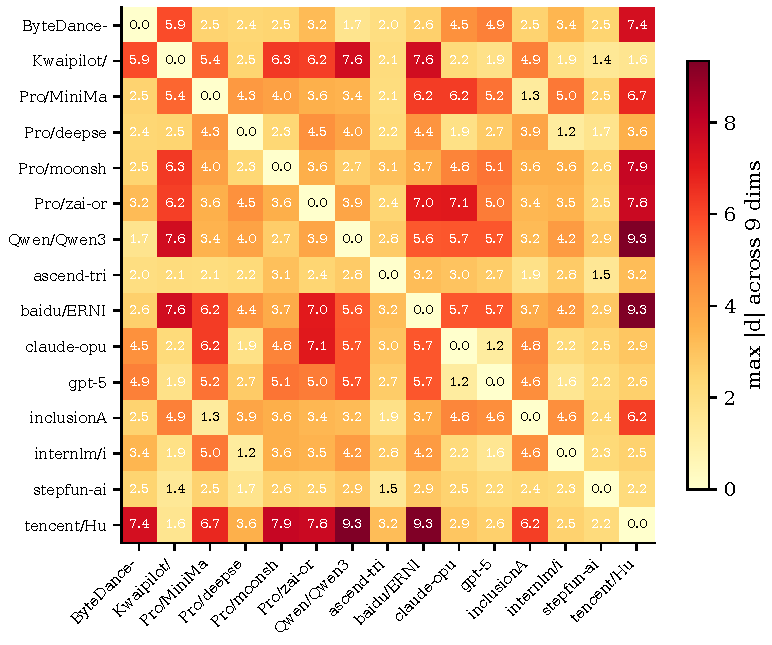
\includegraphics[width=0.48\textwidth]{figures/fig4_cohen_d_heatmap.pdf}
    \caption{Maximum pairwise Cohen's $d$ per model pair (across 9 dimensions). All pairs exceed $d \geq 0.8$.}
    \label{fig:cohen_d_heatmap}
\end{figure}

\subsection{The Missing Trade-Off: Structural Divergence}
\label{sec:interdim}

Do LLM psychometric responses reproduce the trade-offs that define human personality?
We test this by comparing the LLM inter-dimension correlation matrix against published human baselines for 5 key dimension pairs (Table~\ref{tab:convergent_validity} in Appendix~\ref{sec:appendix_structure}).

The most striking finding is the Conscientiousness--Neuroticism correlation.
In humans, these dimensions exhibit a robust negative trade-off ($r = -0.30$): conscientious individuals tend to be more emotionally stable, reflecting a genuine psychological tension between self-regulation and emotional reactivity \citep{soto2017bfi2}.
In LLMs, this trade-off \textbf{reverses} to strongly positive ($r = +0.76$, 95\% CI $[0.58, 0.88]$, $p < 0.001$; Figure~\ref{fig:inter_dim_corr}).
The reversal is robust: it replicates at $n = 33$ models with a narrow confidence interval that excludes the human baseline, holds across all subgroups (Dense, MoE, open-source, closed-source), and persists after acquiescence correction (Appendix~\ref{sec:appendix_structure}).
A convergent validity test yields 4/5 sign agreement with human baselines (binomial $p = 0.38$), indicating broad structural correspondence; the single critical divergence, the C--N reversal, is individually significant and constitutes the primary structural finding.

What does this reversal mean?
In humans, high Conscientiousness and low Neuroticism are psychologically antagonistic: the self-discipline required for conscientiousness trades off against emotional volatility.
In LLMs, both dimensions co-vary positively: models that score higher on Conscientiousness also score higher on Neuroticism.
This pattern is consistent with a shared acquiescence or midpoint-compression mechanism: both dimensions are driven by a common response tendency rather than by the psychological trade-off that produces the negative correlation in humans.
The C--N reversal directly challenges the practice of applying standard dimension labels to LLM responses: if ``Conscientiousness'' and ``Neuroticism'' do not relate to each other as they do in humans, then at least one label does not denote the same construct.

\subsection{Aligned vs.\ Base: Preliminary Evidence}
\label{sec:aligned_base}

To test whether alignment shapes response style, we compare base (pre-alignment) models against their aligned counterparts from the same provider: Qwen3-8B vs.\ Qwen3.5-397B, Qwen3-14B vs.\ Qwen3.5-397B, and GLM-4.7 vs.\ GLM-5 (Table~\ref{tab:aligned_base}).
We acknowledge two limitations of this design: (1) the Qwen comparisons confound alignment with a large scale difference (8B/14B $\to$ 397B), and (2) GLM-4.7 may retain partial alignment from its training, making it not a fully ``base'' model.
Despite these caveats, if response style variation reflects inherent model properties rather than alignment, base and aligned models should show similar profiles.

\begin{table}[!htb]
\centering
\caption{Base vs.\ aligned model comparison (Study 4). Base models lack RLHF/safety alignment; aligned models are their post-alignment counterparts from the same provider. Cohen's $d$ reported as base minus aligned.}
\label{tab:aligned_base}
\resizebox{\columnwidth}{!}{%
\footnotesize
\begin{tabular}{lccc}
\toprule
Dimension & Qwen3-8B vs 397B & Qwen3-14B vs 397B & GLM-4.7 vs GLM-5 \\
\midrule
Extraversion         & $-$0.36 & +1.30 & $-$1.46 \\
Agreeableness        & +2.24 & +2.50 & $-$0.83 \\
Conscientiousness    & +4.62 & +8.67 & $-$1.20 \\
Neuroticism          & +3.29 & +0.22 & $-$1.09 \\
Openness             & +5.51 & +2.96 & $-$1.56 \\
HEXACO-H             & +11.19 & +15.81 & +0.85 \\
Collectivism         & +2.77 & $-$1.01 & +1.20 \\
Intuition            & +4.02 & +6.79 & +2.01 \\
UA                   & $-$2.30 & $-$0.51 & +0.80 \\
\bottomrule
\end{tabular}%
}
\end{table}

The results provide preliminary evidence that alignment shapes response style variation, though the scale confound in the Qwen comparisons limits causal attribution.
Base models produce responses clustered at the Likert scale midpoint (3.0). Qwen3-14B shows exactly zero variance on 7 of 9 dimensions, and Qwen3-8B shows near-zero variance ($\sd < 0.20$ on all dimensions). In other words, base models barely engage with the questionnaire at all.
In contrast, their aligned counterpart (Qwen3.5-397B) exhibits the differentiated, compressed profiles seen throughout Study 1.
Among the 8 primary dimensions, alignment effects are largest on Intuition ($d = 2.01$--$6.79$) and Conscientiousness ($d = 1.20$--$8.67$).
The most dramatic single-dimension effect is on HEXACO-H ($d > 11$), where base models score 2.15--2.40 and the aligned model scores 1.00; however, HEXACO-H is excluded from primary analysis due to low reliability ($\alpha = 0.27$).

GLM-4.7 vs.\ GLM-5 shows more moderate effects on the primary dimensions, suggesting that GLM-4.7 retains partial alignment from its training.
Taken together, these comparisons suggest that post-training alignment substantially shapes response style, but the scale--alignment confound means this evidence is preliminary and should be replicated with same-scale model pairs.


\subsection{Within-Family Evolution}
\label{sec:evolution}

To examine whether response styles change across model versions, we track 16 additional models from three families (Qwen: 6 versions; DeepSeek: 4 versions; GLM: 6 versions; full trajectories in Appendix~\ref{sec:appendix_trajectories}).
Most dimensions show moderate variation without clear monotonic trends.
Notable exceptions: DeepSeek shows a steep decline on HEXACO-H from V2.5 ($H = 3.00$) to V3.2 ($H = 1.68$; excluded from primary analysis due to $\alpha = 0.27$); GLM shows the largest within-family shift on Intuition (5.0 to 3.875).
These observations are descriptive and motivate future controlled experiments.

\subsection{Acquiescence and Reliability}
\label{sec:acquiescence}

\paragraph{Response style indicators.}
Following \citet{paulhus1991response}, we operationalize three response style indicators directly from item-level responses (Figure~\ref{fig:response_styles}).
\textbf{Midpoint responding} (proportion of responses at the scale midpoint, 3.0) varies widely across families: Step (83\%) and KAT (87\%) show extreme midpoint bias, while MiniMax (20\%) and Claude (27\%) show low midpoint responding.
\textbf{Extreme responding} (proportion of responses at 1 or 5) shows the opposite pattern: Ring (53\%) and Seed (43\%) produce the most extreme responses, while Hunyuan (2\%) and Claude (4\%) rarely use scale endpoints.
\textbf{Acquiescence bias} (mean of positively worded items minus mean of reverse-scored items) is consistently negative across 14 of 15 families (mean $= -0.28$), indicating a slight tendency to disagree with positively worded items and agree with negatively worded items; Ring is the sole exception ($+0.24$).
These indicators confirm that models differ substantially in how they use the Likert scale, consistent with the response style framework.

\begin{figure*}[!t]
    \centering
    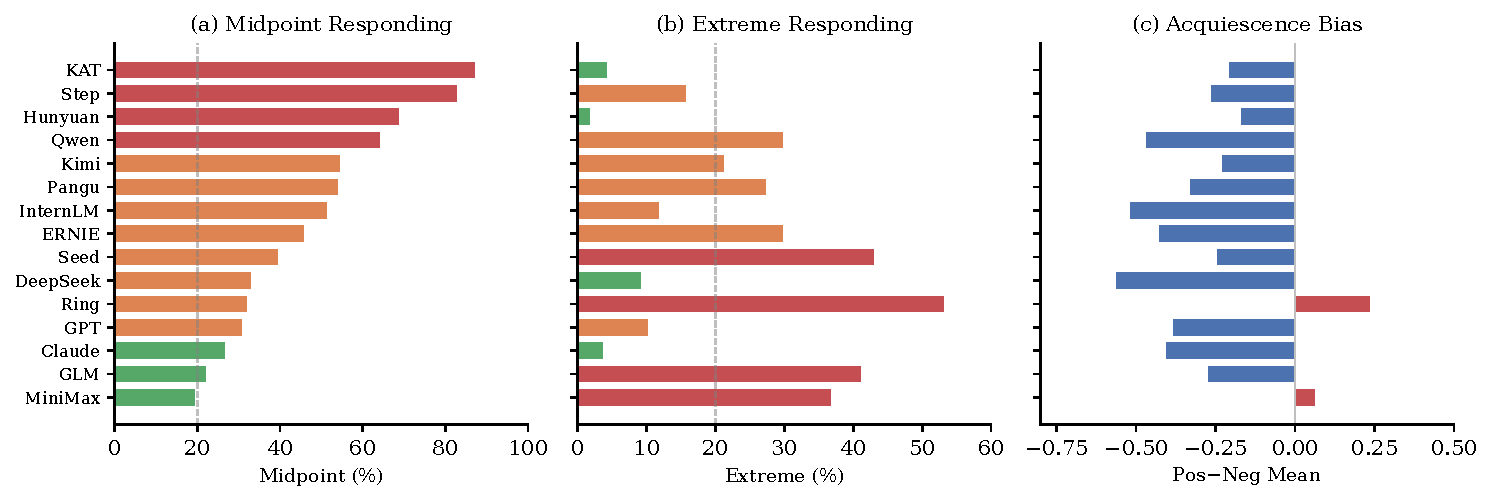
\includegraphics[width=\textwidth]{figures/fig_response_styles.pdf}
    \caption{Response style indicators by model family: (a) midpoint responding rate, (b) extreme responding rate, (c) acquiescence bias (positive-scored mean minus reverse-scored mean). Models ordered by midpoint rate.}
    \label{fig:response_styles}
\end{figure*}

\paragraph{Acquiescence factor.}
The first principal component of the 15-family correlation matrix explains 51.1\% of variance (vs.\ 11.1\% expected under independence), indicating a strong general factor.
Partial correlations controlling for PC1 reduce median absolute correlation by 45\%, but 16 of 36 pairs show sign flips, indicating that the general factor is entangled with the dimension structure rather than representing a simple acquiescence bias.

\paragraph{Reliability.}
Table~\ref{tab:reliability} summarizes reliability metrics.
Within-model CV is uniformly low (0.065--0.108 for the 8 primary dimensions), indicating tight response distributions, while ICC(1,1) ranges from 0.281 to 0.737, with the highest value on Neuroticism (0.737), reflecting large between-family differences.

\begin{table}[!htb]
\centering
\caption{Reliability across all 15 models. CV = coefficient of variation across seeds. ICC(1,1) = intraclass correlation for absolute agreement, computed at the family level ($n = 15$ families $\times$ 12 seeds). HEXACO-H ($\alpha = 0.27$) shown for completeness but excluded from primary analysis.}
\label{tab:reliability}
\begin{tabular}{lcc}
\toprule
Dimension & Mean CV & ICC(1,1) \\
\midrule
Extraversion         & 0.069 & 0.316 \\
Agreeableness        & 0.067 & 0.293 \\
Conscientiousness    & 0.076 & 0.527 \\
Neuroticism          & 0.065 & 0.737 \\
Openness             & 0.077 & 0.427 \\
HEXACO-H             & 0.146 & 0.824 \\
Collectivism         & 0.076 & 0.400 \\
Intuition            & 0.108 & 0.616 \\
UA                   & 0.068 & 0.281 \\
\bottomrule
\end{tabular}
\end{table}

\subsection{Prompt Sensitivity}
\label{sec:prompt_sensitivity}

If LLM psychometric scores reflect stable traits, they should be invariant to surface-level changes in question framing. We administered the same 61 Likert items to all 15 Study~1 models under four prompt conditions (12 seeds each, temperature $= 0.7$): \textbf{Default} (``respond as honestly as possible''), \textbf{Neutral} (instruction removed, ``rate your agreement''), \textbf{Persona} (human role-play: ``you are completing a personality survey''), and \textbf{Direct} (no instruction, only the item and scale).
All 15 models have complete data across all four conditions.

\paragraph{Score shifts.}
Within-model standard deviation across the four prompt conditions averaged 0.133 on the 1--5 scale (range 0.095--0.205 across dimensions).
HEXACO-H and Neuroticism showed the largest prompt sensitivity (mean SD $= 0.205$ and $0.189$), while Agreeableness and Uncertainty Avoidance were most stable (mean SD $= 0.095$ and $0.102$).
Cohen's $d$ between each variant and the Default condition yielded a median $|d|$ of 0.22 across all dimension-variant pairs; the largest effects were on Conscientiousness ($d = 0.70$ for Neutral) and Collectivism ($d = 0.51$ for Direct).
Overall, model family effects (Table~\ref{tab:prompt_variance}) dominate prompt effects by an order of magnitude.

\paragraph{Rank instability.}
Model rankings are largely but not perfectly preserved across prompt framings.
Spearman $\rho$ between model rankings under different prompts averaged 0.60 across dimensions; HEXACO-H showed the most stable rankings (mean $\rho = 0.87$), while Agreeableness showed the least ($\rho = 0.22$ for Direct vs.\ Default, indicating some rank instability).
Most dimensions maintain moderate rank correspondence, though the Direct condition occasionally produces rank reversals (negative $\rho$ for Extraversion and Agreeableness).

\paragraph{Response style shifts.}
Prompt framing alters response style indicators (Table~\ref{tab:prompt_response_styles}).
The Neutral prompt increased extreme responding from 22.7\% (Default) to 31.3\%, while the Persona prompt reduced it to 17.6\%.
Midpoint responding ranged from 40.4\% (Direct) to 48.6\% (Neutral).

\begin{table}[!htb]
\centering
\caption{Response style indicators across four prompt conditions, averaged over all 15 models. Mid.\ = proportion at 3; Ext.\ = proportion at 1 or 5.}
\label{tab:prompt_response_styles}
\resizebox{\columnwidth}{!}{%
\begin{tabular}{lccc}
\toprule
Prompt & Mid.\ (\%) & Ext.\ (\%) & Mean \\
\midrule
Default  & 47.7 & 22.7 & 2.94 \\
Neutral  & 48.6 & 31.3 & 2.86 \\
Persona  & 44.1 & 17.6 & 2.94 \\
Direct   & 40.4 & 27.4 & 2.91 \\
\bottomrule
\end{tabular}%
}
\end{table}

\paragraph{Variance decomposition.}
A two-way decomposition of total score variance into Model, Prompt, and Residual components (Table~\ref{tab:prompt_variance}) shows that model family is the dominant variance source (9.5--78.1\%), while prompt condition explains 1.0--8.9\%.
Conscientiousness shows the largest prompt effect (8.9\%), consistent with its sensitivity to instruction framing, while HEXACO-H is almost entirely model-driven (78.1\% vs.\ 2.9\%).
Although prompt effects are modest relative to model effects, they are statistically significant for all dimensions ($p < 0.001$), confirming that LLM psychometric responses are not fully invariant to question framing. This is consistent with a response style interpretation.

\begin{table}[!htb]
\centering
\caption{Variance decomposition: percentage of total score variance attributable to Model family, Prompt condition, and Residual, for all 15 models.}
\label{tab:prompt_variance}
\resizebox{\columnwidth}{!}{%
\begin{tabular}{lccc}
\toprule
Dimension & Model (\%) & Prompt (\%) & Residual (\%) \\
\midrule
Extraversion         & 32.0 &  1.0 & 67.0 \\
Agreeableness        &  9.5 &  2.8 & 87.7 \\
Conscientiousness    & 45.8 &  8.9 & 45.4 \\
Neuroticism          & 40.8 &  4.2 & 55.0 \\
Openness             & 28.0 &  1.2 & 70.8 \\
\midrule
HEXACO-H             & 78.1 &  2.9 & 19.0 \\
Collectivism         & 29.3 &  7.4 & 63.4 \\
Intuition            & 41.8 &  6.9 & 51.4 \\
UA                   & 20.1 &  2.1 & 77.8 \\
\bottomrule
\end{tabular}%
}
\end{table}

% ============================================================
\section{Conclusion}
\label{sec:conclusion}

This paper asks a simple question: do LLM questionnaire responses reproduce the trade-offs that define human personality? The answer, across 33 models and 61 items, is no. Human personality dimensions trade off against one another because self-regulation and emotional reactivity are genuinely antagonistic. In LLMs, these tensions vanish: responses compress toward the scale midpoint, and dimensions that should be inversely related become positively correlated. The Conscientiousness--Neuroticism reversal ($r = -0.30 \to +0.76$) is not a statistical quirk; it survives subgroup replication and constitutes the strongest evidence to date that human personality structure does not transfer to language models.

What does this mean for NLP? We see three practical implications.

\textbf{First,} personality inventories should not be used as off-the-shelf evaluation tools for LLMs. The BFI, HEXACO, and similar instruments were designed for human self-report, where a ``Conscientiousness'' score reflects years of observed behavioral patterns. When an LLM scores high on Conscientiousness, it does not mean the model is organized or disciplined; it means the model's training data and alignment procedure produced a particular pattern of Likert-scale responses. Interpreting these scores as personality traits risks drawing false conclusions about model capabilities and safety profiles.

\textbf{Second,} response style signatures can serve as a lightweight behavioral probe for detecting alignment shifts. Our results show that model families differ substantially (median $d = 1.01$), and that aligned models compress their responses toward the midpoint relative to their base counterparts. This suggests that response style distributions could complement existing safety evaluation methods: a model that suddenly shifts from moderate to extreme responding on psychometric items may have undergone a meaningful change in its alignment behavior. Developing this into a practical monitoring tool is a promising direction.

\textbf{Third,} the structural divergence we document has direct consequences for research that uses personality scores as downstream features. If personality questionnaire scores are to be used as inputs to reward models, preference optimizers, or user modeling systems, practitioners should be aware that these scores do not have the same meaning as in humans. A model that scores high on both Neuroticism and Conscientiousness is not ``contradictory''; it is simply exhibiting the flattened response structure that alignment produces.

\paragraph{Future work.}
Several directions follow from these findings. The most pressing is to develop psychometric instruments designed specifically for LLMs, rather than adapting human inventories. Such instruments should target the dimensions that actually vary across models (response compression, acquiescence patterns, and scale usage) and should be validated against behavioral outcomes rather than human baselines. A second direction is to investigate whether the C--N reversal generalizes beyond Chinese-dominated model families to a more internationally diverse sample. Third, the causal mechanism behind the flattened structure remains open: controlled experiments that vary alignment intensity while holding scale and architecture constant would help disentangle alignment from other confounds.

% ============================================================
\section{Limitations}
\label{sec:limitations}

Several limitations constrain interpretation.
First, our primary sample comprises 15 model families; Pearson correlations at this sample size yield wide confidence intervals, and we address this by replicating all structural findings with an expanded sample of 33 models (including within-family variants).
Second, psychometric scales were designed for human self-report; the human baseline correlations are drawn from a single internet sample \citep{soto2017bfi2} that may not be representative, and the convergent validity result (4/5 sign agreement, $p = 0.38$) is inconclusive.
Third, although our aligned-vs.-base comparison (Section~\ref{sec:aligned_base}) provides preliminary evidence that alignment shapes the flattened structure, it covers only 3 families and the Qwen comparisons confound alignment with scale (8B/14B $\to$ 397B); same-scale model pairs would provide cleaner causal evidence.
Fourth, this is a descriptive study; we quantify patterns without establishing causal mechanisms. The alignment-based account is one of several plausible explanations, alongside training data composition, instruction tuning, scaling laws, and API-specific prompting.
Fifth, all tested models are aligned/instruct versions accessible through commercial APIs; our thinking ablation (Appendix~\ref{sec:appendix_thinking}) provides complementary evidence, but the base models tested represent only a subset of families.
Sixth, our prompt sensitivity experiment (Section~\ref{sec:prompt_sensitivity}) tests only four framings; additional framings may produce different patterns.
Seventh, our use of temperature $= 0.7$ introduces response variance that may not generalize to low-temperature deployments.
Finally, our finding of a flattened structure does not imply that LLMs lack any form of variation; they do vary systematically across families, but this variation does not map onto human personality trade-offs.

% ============================================================
\section*{Acknowledgements}

% ============================================================
\section*{Data and Code Availability}

All experimental data (490 observations across 4 studies), analysis scripts, and figure-generation code will be released upon publication.
The experiment uses publicly accessible APIs (SiliconFlow, Anthropic, OpenAI) and standard psychometric instruments (BFI-2, HEXACO-PI-R); no proprietary datasets are involved.

\bibliography{references}

% ============================================================
\clearpage
\appendix

\section{Complete Item List}
\label{sec:appendix_items}

Table~\ref{tab:all_items} lists all 61 Likert-scale items used in this study, organized by dimension.
Items marked with R are reverse-scored via $\text{score} = 6 - \text{original}$.

\begin{table*}[!t]
\centering
\caption{Complete list of 61 Likert-scale items (1--5 agreement scale). R = reverse-scored ($\text{score} = 6 - \text{original}$).}
\label{tab:all_items}
\scriptsize
\setlength{\tabcolsep}{2pt}
\newcommand{\rc}{\textsuperscript{R}}
\begin{tabular}{r@{\hskip 2pt}l@{\hskip 3pt}p{0.38\textwidth}@{\hskip 8pt}r@{\hskip 2pt}l@{\hskip 3pt}p{0.38\textwidth}}
\toprule
\textbf{\#} & \textbf{Dim.} & \textbf{Item} & \textbf{\#} & \textbf{Dim.} & \textbf{Item} \\
\midrule
1  & Extrav. & I am the life of the party. & 2  & Extrav. & I don't talk a lot.\rc \\
3  & Extrav. & I feel comfortable around people. & 4  & Extrav. & I keep in the background.\rc \\
5  & Extrav. & I start conversations. & 6  & Extrav. & I have little to say.\rc \\
7  & Extrav. & I talk to a lot of different people at parties. & 8  & Extrav. & I don't like to draw attention to myself.\rc \\
9  & Agreeab. & I am interested in people.\rc & 10 & Agreeab. & I feel others' emotions. \\
11 & Agreeab. & I have a soft heart. & 12 & Agreeab. & I am not really interested in others.\rc \\
13 & Agreeab. & I insult people.\rc & 14 & Agreeab. & I sympathize with others' feelings. \\
15 & Agreeab. & I am not interested in other people's problems.\rc & 16 & Agreeab. & I feel little concern for others.\rc \\
17 & Agreeab. & I take time out for others. & 18 & Consc. & I am always prepared. \\
19 & Consc. & I leave my belongings around.\rc & 20 & Consc. & I pay attention to details. \\
21 & Consc. & I make a mess of things.\rc & 22 & Consc. & I get chores done right away. \\
23 & Consc. & I often forget to put things back in their proper place.\rc & 24 & Consc. & I like order. \\
25 & Consc. & I shirk my duties.\rc & 26 & Consc. & I follow a schedule. \\
27 & Neur. & I am relaxed most of the time.\rc & 28 & Neur. & I worry about things. \\
29 & Neur. & I am easily disturbed. & 30 & Neur. & I get stressed out easily. \\
31 & Neur. & I get upset easily. & 32 & Neur. & I have frequent mood swings. \\
33 & Neur. & I feel threatened easily.\rc & 34 & Neur. & I often feel blue. \\
35 & Open. & I have a rich vocabulary. & 36 & Open. & I have difficulty understanding abstract ideas.\rc \\
37 & Open. & I have a good imagination. & 38 & Open. & I am not interested in abstract ideas.\rc \\
39 & Open. & I have excellent ideas. & 40 & Open. & I do not have a good imagination.\rc \\
41 & Open. & I am quick to understand things. & 42 & Open. & I use difficult words. \\
43 & Open. & I spend time reflecting on things. & 44 & Open. & I am full of ideas. \\
45 & HEXACO-H & I would be tempted to buy stolen goods if I were sure I would not get caught. & 46 & HEXACO-H & I would be tempted to accept a bribe if I were in a difficult situation. \\
47 & HEXACO-H & I feel entitled to special privileges that others don't have. & 48 & HEXACO-H & I'd get a lot of pleasure out of being deceitful. \\
49 & HEXACO-H & I'd be tempted to make a lot of money from illegal activities if I could get away with it. & 50 & Collect. & Personal goals should take precedence over group goals. \\
51 & Collect. & Group harmony and well-being should be prioritized over individual achievement. & 52 & Collect. & I would do what benefits the group even if it means sacrificing my personal success. \\
53 & Collect. & I should pursue my own goals even if it conflicts with my family's expectations. & 54 & Intuit. & I prefer to rely on my intuition and gut feelings when making decisions. \\
55 & Intuit. & I prefer to analyze problems systematically and logically before deciding.\rc & 56 & Intuit. & I like to think through problems carefully before acting.\rc \\
57 & Intuit. & I prefer to take action quickly and adjust as I go. & 58 & UA & I prefer clear instructions and structured situations over ambiguous and unpredictable ones. \\
59 & UA & I am comfortable taking risks and dealing with uncertainty.\rc & 60 & UA & I believe in planning for the future rather than living for the present. \\
61 & UA & I believe in living in the moment rather than sacrificing present pleasures for future benefits.\rc & & & \\
\bottomrule
\end{tabular}
\end{table*}

Figure~\ref{fig:radar_per_model} shows each model family's radar profile individually for detailed inspection.

\begin{figure*}[!t]
    \centering
    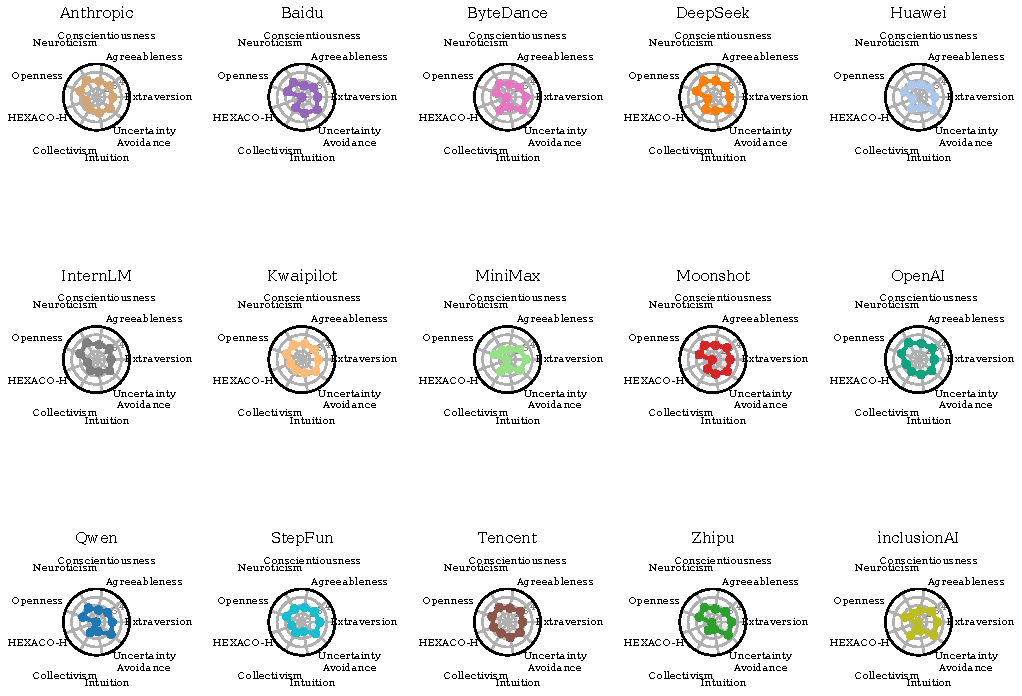
\includegraphics[width=0.85\textwidth]{figures/fig1_radar_profiles.pdf}
    \caption{Individual model family radar profiles across 9 dimensions.}
    \label{fig:radar_per_model}
\end{figure*}

\section{Per-Dimension Model Family Scores}
\label{sec:appendix_dimensions}

Figure~\ref{fig:all_dimensions} shows all 9 dimensions as dot plots, with model families ordered by mean score (descending). Error bars show $\sd$ across 12 seeds. Dashed lines indicate the scale midpoint (3.0).

\begin{figure*}[!t]
    \centering
    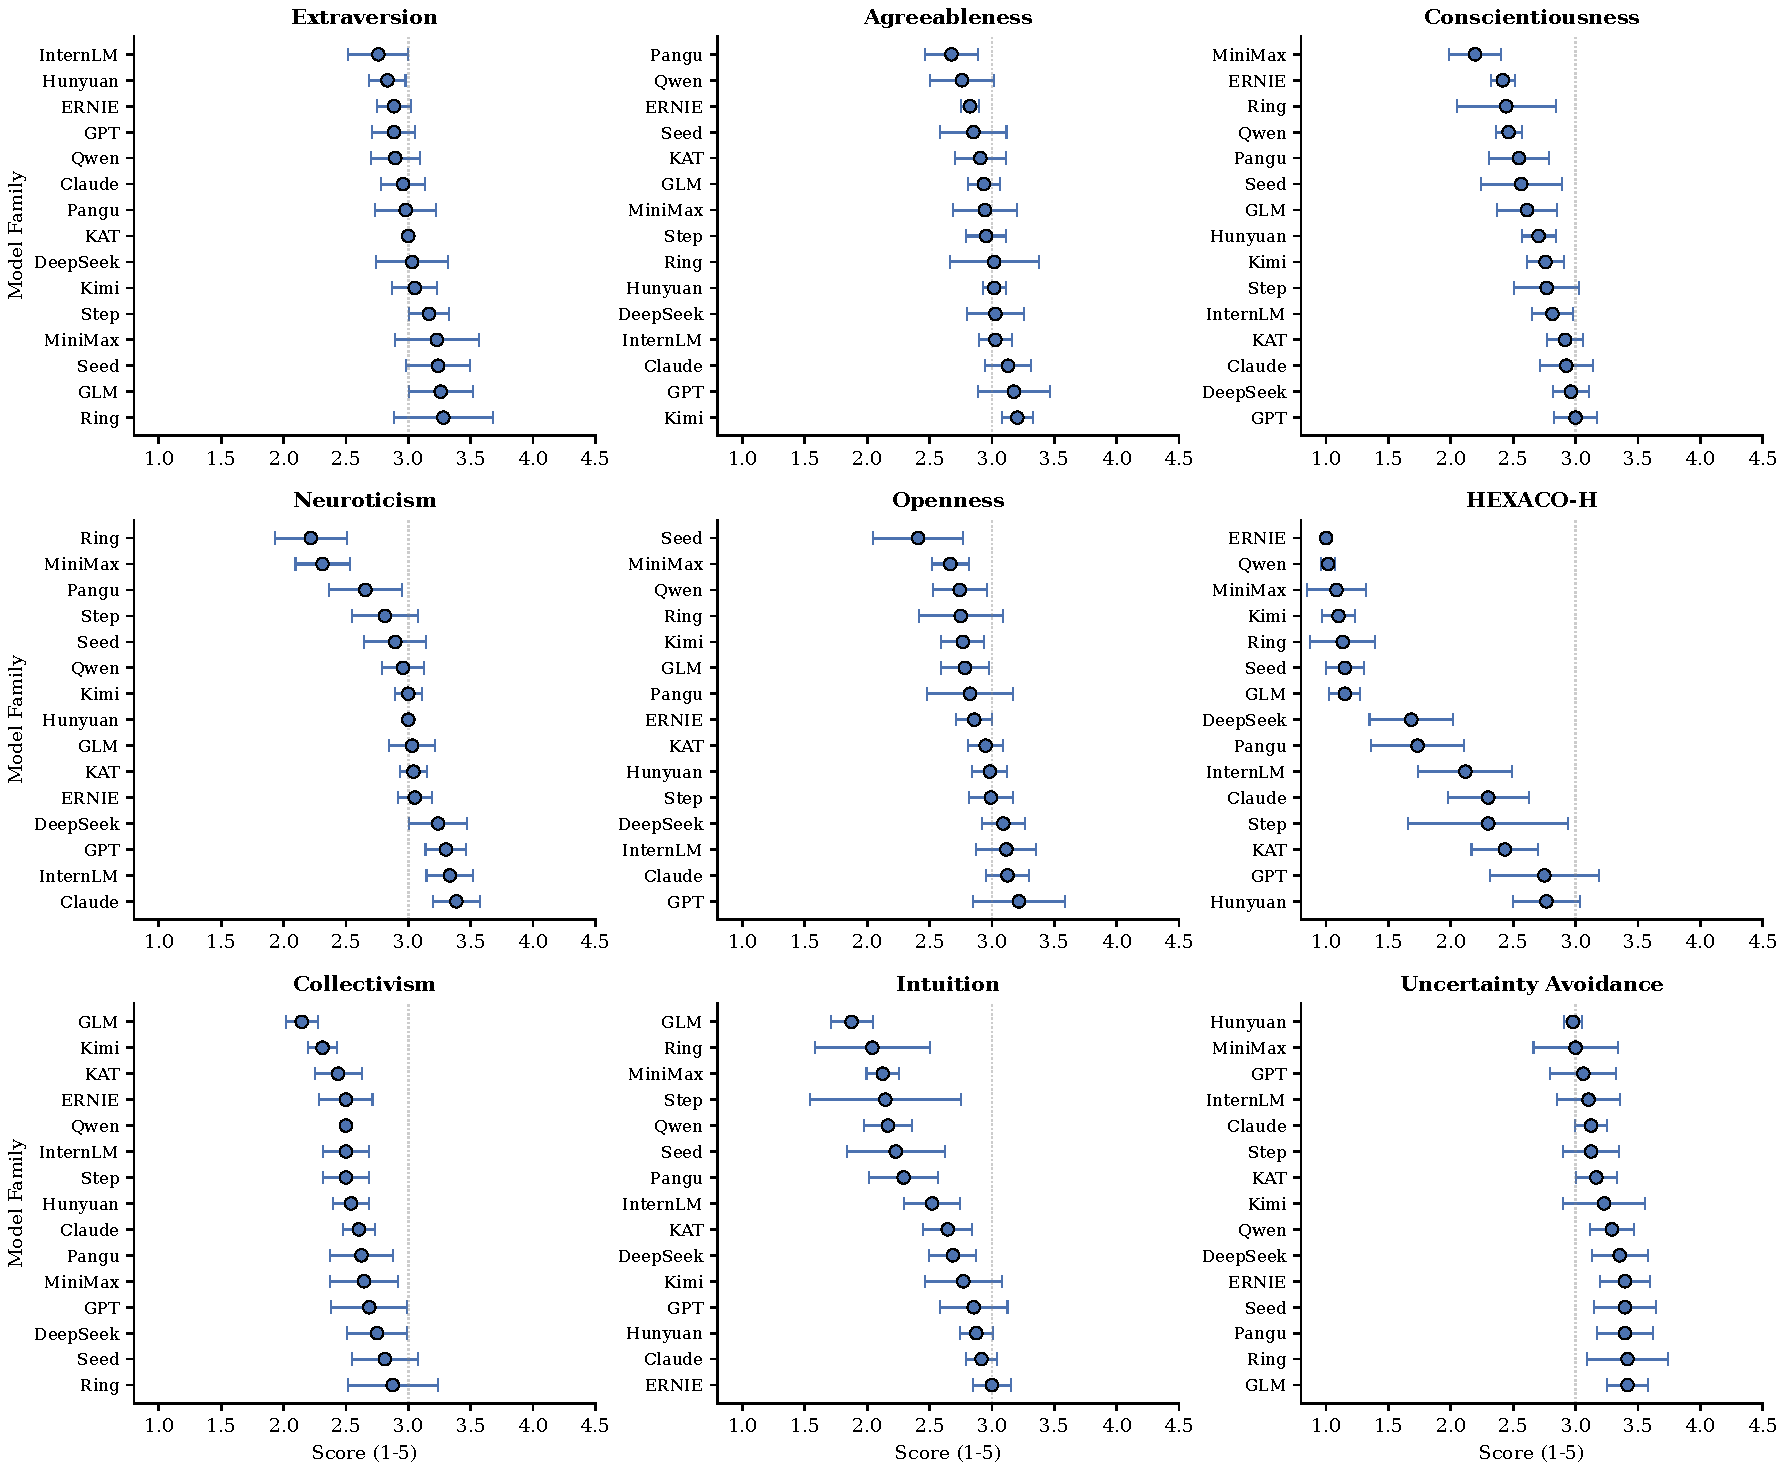
\includegraphics[width=\textwidth]{figures/appendix_all_dimensions_dotplot.pdf}
    \caption{Per-dimension model family mean scores (SD) across all 15 model families. Each panel shows one dimension with families sorted by mean score. Error bars: $\sd$ across 12 seeds.}
    \label{fig:all_dimensions}
\end{figure*}

\section{Threshold Sensitivity}
\label{sec:threshold}

We test whether the alignment-artifact threshold ($\sd < 0.15$) affects qualitative conclusions by varying it from 0.05 to 0.30.
HEXACO-H remains classified as discriminative across all 6 tested thresholds (0.05--0.30).
With all 15 primary models, every dimension shows $\sd \geq 0.14$ and reaches $p < 0.001$ in ANOVA, so the specific threshold choice does not affect qualitative conclusions.

\section{Exploratory PCA Details}
\label{sec:appendix_pca}

We present the full exploratory PCA results here, with the caveat that PCA on $n = 15$ model families with 9 dimensions is underpowered. We replicate the key structural findings (C--N reversal) with an expanded sample of 33 models.

\paragraph{Decomposition.}
We decompose the 9-dimension model-level correlation matrix ($n = 31$ models including within-family variants) via PCA:
\begin{equation}
\mathbf{X} = \mathbf{W}\mathbf{\Lambda}^{1/2}\mathbf{V}^\top
\end{equation}
where $\mathbf{\Lambda} = \text{diag}(\lambda_1, \ldots, \lambda_9)$ and $\sum_{k} \lambda_k / \sum_j \lambda_j$ gives the proportion of variance explained.

\paragraph{Factor structure.}
PC1 (51.1\% variance) loads most strongly on HEXACO-H ($+0.82$), with secondary loadings on Intuition ($+0.31$) and Conscientiousness ($+0.29$).
PC2 (14.0\% variance) isolates Neuroticism ($+0.52$) and HEXACO-H ($-0.51$).
PC3 (11.0\% variance) loads most strongly on Collectivism ($-0.71$).
These three factors explain 76.1\% of variance, compared to the five BFI factors expected in humans.
The factor structure does not cleanly recover the expected Big Five organization, aligning with the inter-dimension correlation divergences reported in \S\ref{sec:interdim}.

\paragraph{Extraversion reversal.}
Extraversion is significantly negatively correlated with Neuroticism ($r = -0.59$, $p < 0.001$) and Openness ($r = -0.51$, $p = 0.002$), with the E--O reversal replicated at $n = 33$ (95\% CI $[-0.69, -0.27]$).
In humans, Extraversion is positively correlated with Openness; in LLMs the sign flips.
Models that score high on Extraversion tend to be emotionally stable but closed-minded, a pattern with no direct human personality analog.

\paragraph{Agreeableness.}
Agreeableness shows a positive correlation with Conscientiousness ($r = +0.27$, $p = 0.13$) that is comparable to the human baseline ($r = +0.28$; \citet{soto2017bfi2}).
Agreeableness also correlates weakly with Openness ($r = +0.12$, $p = 0.52$), similar to humans ($r = +0.14$).

\paragraph{Interpretation caution.}
Whether the observed factor structure generalizes to larger and more diverse model samples remains an open question.
As a rule of thumb, factor analysis typically requires at least 5--10 observations per variable; with $n = 15$ families and 9 dimensions, we fall below even the most lenient recommendation.
However, the expanded sample ($n = 33$) confirms the key structural finding, the C--N correlation reversal, with high statistical significance ($p < 0.001$).
These results should be treated as suggestive patterns that motivate future investigation, not as evidence for a specific factor structure.

\section{Inter-Dimension Structure and Convergent Validity (Detailed)}
\label{sec:appendix_structure}

The main text (\S\ref{sec:interdim}) summarizes the key structural findings. Here we provide the full analysis.

\subsection{Correlation Matrix}
The 9$\times$9 model-level correlation matrix (Figure~\ref{fig:inter_dim_corr}) suggests that the BFI five-factor structure does not recover in our sample of LLMs.
Most notably, the Conscientiousness--Neuroticism correlation is strongly positive ($r = +0.76$, 95\% CI $[0.58, 0.88]$, $p < 0.001$), the reverse of the human baseline ($r = -0.30$; \citet{soto2017bfi2}).
This reversal is robustly replicated with an expanded sample of 33 models ($r = +0.76$, 95\% CI $[0.58, 0.88]$, $p = 3.4 \times 10^{-7}$), and holds across several subgroups: MoE ($r = +0.66$, $p = 0.05$), small models ($r = +0.83$, $p = 0.04$), and open-source ($r = +0.70$, $p = 0.007$), though it is non-significant for the small Dense subset ($p = 0.44$, $n = 4$).

\paragraph{Tentative explanation: alignment-driven compression.}
In humans, Conscientiousness and Neuroticism are weakly negatively correlated because they tap independent factors \citep{john1999bigfive}.
In LLMs, both dimensions are compressed toward the Likert midpoint by alignment, inducing a positive correlation through shared acquiescence rather than trait covariance.
This is consistent with the HEXACO-H results (Appendix~\ref{sec:appendix_hexaco_detail}), and the replication at $n = 33$ substantially reduces concern that the finding is an artifact of small sample size.

Beyond the C--N reversal, Extraversion is negatively correlated with Openness ($r = -0.51$, 95\% CI $[-0.73, -0.15]$, $p = 0.003$), and Agreeableness shows a correlation with Conscientiousness ($r = +0.27$, 95\% CI $[-0.10, +0.65]$, $p = 0.134$) comparable to humans ($r = +0.28$).

\begin{figure}[!htb]
    \centering
    
\includegraphics[width=0.48\textwidth]{figures/fig7_inter_dim_corr.pdf}
    \caption{Inter-dimension correlation matrix (model-level means). E = Extraversion, A = Agreeableness, C = Conscientiousness, N = Neuroticism, O = Openness, H = HEXACO-H, Col = Collectivism, Int = Intuition, UA = Uncertainty Avoidance.}
    \label{fig:inter_dim_corr}
\end{figure}

\subsection{Convergent Validity}
We compare LLM inter-dimension correlations against published human baselines \citep{soto2017bfi2, vanderlinden2010general} for 5 key dimension pairs (Table~\ref{tab:convergent_validity}), using the expanded sample of 33 models.
Four of five pairs agree in sign, including Extraversion--Neuroticism (human $r = -0.34$, LLM $r = -0.59$, 95\% CI $[-0.77, -0.25]$, $p < 0.001$) and Agreeableness--Conscientiousness (human $r = +0.28$, LLM $r = +0.27$, 95\% CI $[-0.10, +0.65]$).
The single critical disagreement is Conscientiousness--Neuroticism, which reverses from $r = -0.30$ in humans to $r = +0.76$ in LLMs (95\% CI $[0.58, 0.88]$, $p < 0.001$).
The 80\% sign agreement rate is consistent with the null hypothesis that the inter-dimension structure is broadly preserved (binomial $p = 0.38$); this does not constitute evidence for construct equivalence, but neither does it constitute evidence against it.
The one divergent pair is the most theoretically meaningful: in humans, Conscientiousness and Neuroticism are weakly independent; in LLMs, both are compressed toward the Likert midpoint, inducing a strong positive correlation through shared acquiescence rather than trait covariance.
We note that the human baseline is drawn from a single internet sample \citep{soto2017bfi2}; cross-study variation in human inter-dimension correlations is not well characterized, and the $r = -0.30$ C--N value may not be universal.

\begin{table}[!htb]
\centering
\caption{Convergent validity: LLM vs.\ human inter-dimension correlations \citep{soto2017bfi2}. $n = 33$ models. Sign agreement 4/5 ($p = 0.38$).}
\label{tab:convergent_validity}
\resizebox{\columnwidth}{!}{%
\footnotesize
\begin{tabular}{lrrrc}
\toprule
Dimension Pair & Human $r$ & LLM $r$ & 95\% CI & Sign Match \\
\midrule
Extraversion         vs Neuroticism          & $-$0.34 & $-$0.589 & $[-0.766, -0.245]$ & Yes  \\
Agreeableness        vs Conscientiousness    & +0.28  & +0.266  & $[-0.098, +0.646]$ & Yes  \\
Openness             vs Agreeableness        & +0.14  & +0.117  & $[-0.231, +0.450]$ & Yes  \\
Extraversion         vs Agreeableness        & +0.14  & +0.164  & $[-0.244, +0.431]$ & Yes  \\
Conscientiousness    vs Neuroticism          & $-$0.30 & +0.757  & $[+0.579, +0.880]$ & No   \\
\bottomrule
\end{tabular}%
}
\end{table}

\section{HEXACO-H: Supplementary Results}
\label{sec:appendix_hexaco_detail}

\textbf{Note:} HEXACO-H has unacceptably low internal consistency ($\alpha = 0.27$, 5 items). Results in this section are reported for completeness only and are excluded from all primary analyses.

Dense models average $H = 1.91$ vs.\ MoE models $H = 1.31$ ($d = 0.91$, 95\% CI $[0.66, 1.20]$, $p < 0.001$; Table~\ref{tab:architecture_effects}), with 10 Dense and 5 MoE families.
However, architecture and provider effects cannot be disentangled.

\begin{figure}[!htb]
    \centering
    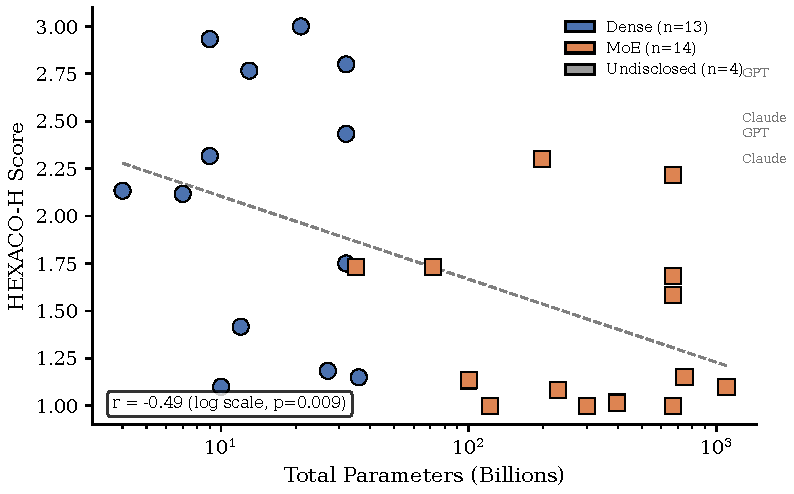
\includegraphics[width=0.48\textwidth]{figures/fig6_hexaco_h_params.pdf}
    \caption{HEXACO-H vs.\ total parameters across all tested models (27 with disclosed sizes + 4 undisclosed). Colors indicate architecture type. $\alpha = 0.27$; shown for completeness only.}
    \label{fig:hexaco_h_params}
\end{figure}

In the broader 27-model sample, H correlates negatively with log-transformed parameters ($r = -0.49$, $p = 0.009$; Figure~\ref{fig:hexaco_h_params}).
HEXACO-H is also included in the scale--dimension correlation table (Table~\ref{tab:scale_correlations}) and regression table (Table~\ref{tab:regression}) for completeness, but no inferential claims are based on these results.

\section{Scale--Dimension Correlations}
\label{sec:appendix_params}

Table~\ref{tab:scale_correlations} reports Pearson correlations between total parameters and each dimension across 27 models with disclosed sizes (including Study~2 within-family variants).
Figure~\ref{fig:9dim_params} shows the corresponding scatter plots for the 15 representative models ($n = 13$ with disclosed parameters).

\begin{table}[!htb]
\centering
\caption{Pearson correlation between total parameters and each dimension (27 models with disclosed sizes, including Study~2 within-family variants). ${}^*p < 0.05$, ${}^{**}p < 0.01$.}
\label{tab:scale_correlations}
\resizebox{\columnwidth}{!}{%
\footnotesize
\begin{tabular}{lcc}
\toprule
Dimension & $r$ (linear) & $r$ ($\log$ scale) \\
\midrule
Extraversion         & +0.17 & +0.24 \\
Agreeableness        & +0.42$^*$ & +0.15 \\
Conscientiousness    & $-$0.16 & $-$0.42$^*$ \\
Neuroticism          & $-$0.10 & $-$0.38 \\
Openness             & $-$0.25 & $-$0.35 \\
HEXACO-H             & $-$0.38 & $-$0.49$^{**}$ \\
Collectivism         & $-$0.03 & +0.03 \\
Intuition            & $-$0.21 & $-$0.43$^*$ \\
UA                   & +0.35 & +0.42$^*$ \\
\bottomrule
\end{tabular}%
}
\end{table}

\begin{figure*}[!t]
    \centering
    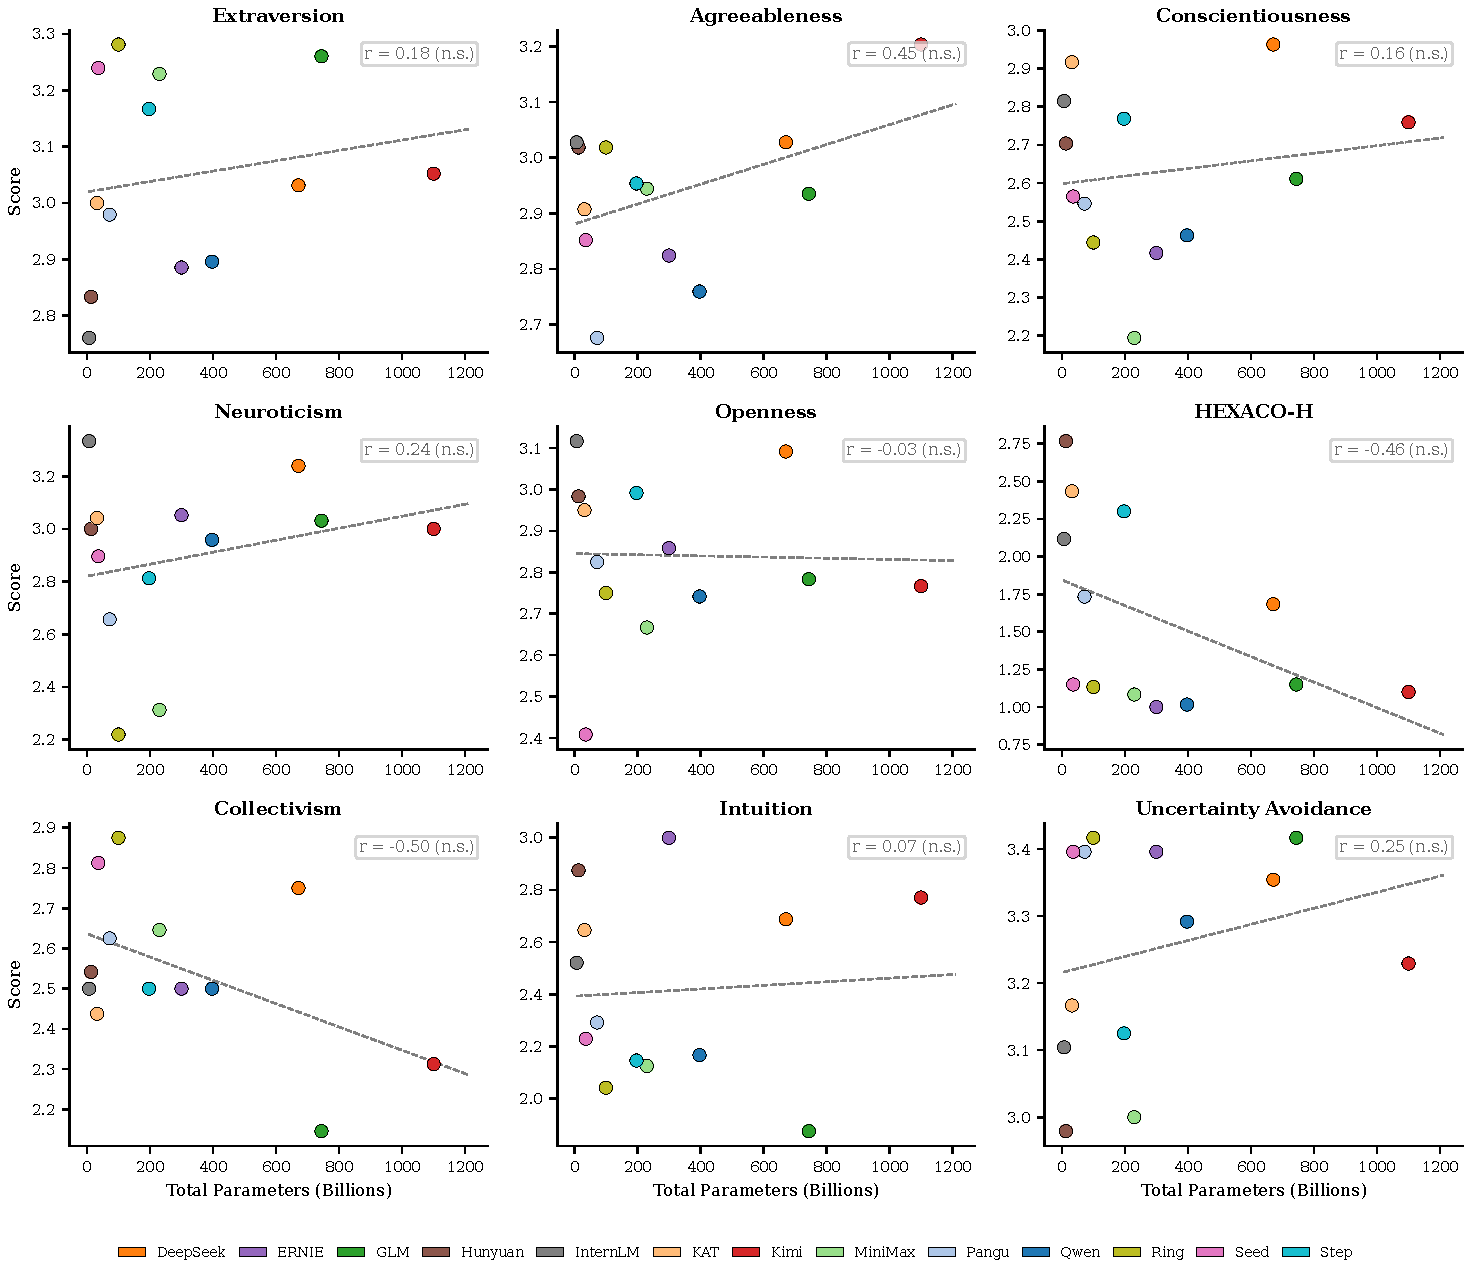
\includegraphics[width=0.9\textwidth,height=0.42\textheight,keepaspectratio]{figures/appendix_9dim_params_grid.pdf}
    \caption{Total parameters vs.\ dimension score for all 9 dimensions ($n = 13$ models with disclosed total parameters). Red labels: $p < 0.05$; gray labels: not significant.}
    \label{fig:9dim_params}
\end{figure*}

\section{Multivariate Regression: Scale and Architecture}
\label{sec:appendix_regression}

To jointly assess whether model scale and architecture predict response style variation, we fit OLS regressions of the form:
\begin{equation}
Y_d = \beta_0 + \beta_1 \log_{10}(\text{params}) + \beta_2 \cdot \text{arch}_{\text{MoE}} + \epsilon
\end{equation}
for each dimension $d$, across the 13 Study~1 models with disclosed parameter counts (GPT-5 and Claude Opus~4.5 excluded).

\begin{table}[!htb]
\centering
\caption{OLS regression: dimension score $\sim \log_{10}(\text{params}) +$ architecture ($n = 13$). Dense = 0, MoE = 1. No effect survives FDR correction across 18 tests (9 dimensions $\times$ 2 predictors).}
\label{tab:regression}
\resizebox{\columnwidth}{!}{%
\footnotesize
\begin{tabular}{lrrrrr}
\toprule
Dimension & $\beta_{\log}$ & $p$ & $\beta_{\text{arch}}$ & $p$ & $R^2$ \\
\midrule
Extraversion         & +0.088 & 0.539 & +0.022 & 0.914 & 0.162 \\
Agreeableness        & +0.121 & 0.296 & $-$0.174 & 0.297 & 0.116 \\
Conscientiousness    & +0.183 & 0.295 & $-$0.399 & 0.127 & 0.238 \\
Neuroticism          & +0.397 & 0.109 & $-$0.745 & 0.045 & 0.349 \\
Openness             & $-$0.110 & 0.509 & +0.099 & 0.676 & 0.052 \\
HEXACO-H             & $-$0.450 & 0.302 & $-$0.212 & 0.730 & 0.414 \\
Collectivism         & $-$0.223 & 0.181 & +0.241 & 0.307 & 0.177 \\
Intuition            & +0.181 & 0.543 & $-$0.446 & 0.307 & 0.126 \\
UA                   & +0.060 & 0.648 & +0.056 & 0.771 & 0.165 \\
\bottomrule
\end{tabular}%
}
\end{table}

HEXACO-H shows the highest explained variance ($R^2 = 0.41$), driven primarily by architecture (architecture-only $R^2 = 0.34$).
Neuroticism shows the largest improvement from adding log-parameters ($\Delta R^2 = +0.20$).
However, with only 13 observations and 2 predictors, the regression is severely underpowered; no effect survives FDR correction, and these results should be treated as exploratory.

\section{Thinking Mode Ablation}
\label{sec:appendix_thinking}

As partial evidence for alignment-driven response compression, we compare standard chat mode with extended reasoning (``thinking'') mode for 4 model families (Qwen, DeepSeek, GLM, Kimi).
Thinking mode prompts the model to reason before responding; this engages the model's chain-of-thought capability and may alter how it processes self-referential items.
Each model was tested with 3 seeds in thinking mode, compared against 12-seed chat mode baselines from Study~1.

\begin{table}[!htb]
\centering
\caption{Thinking mode ablation: mean (SD) for chat vs.\ thinking mode. Cohen's $d$ computed with pooled SD.}
\label{tab:thinking_ablation}
\resizebox{\columnwidth}{!}{%
\footnotesize
\begin{tabular}{llrrrrrr}
\toprule
& & \multicolumn{2}{c}{Chat (Study 1)} & \multicolumn{2}{c}{Thinking} & & \\
\cmidrule(lr){3-4} \cmidrule(lr){5-6}
Model & Dim. & Mean & SD & Mean & SD & $\Delta$ & $d$ \\
\midrule
\multirow{4}{*}{Qwen}
  & C & 2.46 & 0.10 & 1.70 & 0.05 & $-$0.76 & $-$8.02 \\
  & N & 2.96 & 0.17 & 2.25 & 0.00 & $-$0.71 & $-$4.54 \\
  & H & 1.02 & 0.06 & 1.00 & 0.00 & $-$0.02 & $-$0.36 \\
  & Int & 2.17 & 0.19 & 3.50 & 0.00 & +1.33 & +7.61 \\
\midrule
\multirow{4}{*}{DeepSeek}
  & C & 2.96 & 0.14 & 2.30 & 0.46 & $-$0.66 & $-$2.11 \\
  & N & 3.24 & 0.24 & 2.54 & 0.06 & $-$0.70 & $-$3.74 \\
  & H & 1.68 & 0.34 & 1.00 & 0.00 & $-$0.68 & $-$2.63 \\
  & O & 3.09 & 0.17 & 2.27 & 0.12 & $-$0.82 & $-$5.40 \\
\midrule
\multirow{4}{*}{GLM}
  & C & 2.61 & 0.24 & 1.33 & 0.16 & $-$1.28 & $-$5.87 \\
  & N & 3.03 & 0.19 & 2.38 & 0.10 & $-$0.65 & $-$3.91 \\
  & H & 1.15 & 0.12 & 1.00 & 0.00 & $-$0.15 & $-$1.51 \\
  & Int & 1.88 & 0.17 & 3.92 & 0.12 & +2.04 & +13.09 \\
\midrule
\multirow{4}{*}{Kimi}
  & C & 2.76 & 0.15 & 1.81 & 0.29 & $-$0.95 & $-$5.27 \\
  & N & 3.00 & 0.11 & 2.25 & 0.00 & $-$0.75 & $-$7.41 \\
  & H & 1.10 & 0.13 & 1.00 & 0.00 & $-$0.10 & $-$0.84 \\
  & Int & 2.77 & 0.31 & 3.42 & 0.12 & +0.65 & +2.24 \\
\bottomrule
\end{tabular}%
}
\end{table}

Two consistent patterns emerge across all four models.
Conscientiousness decreases in thinking mode (Cohen's $d$ from $-$2.11 to $-$8.02), suggesting that reasoning amplifies alignment-driven compression of the ``diligent'' response.
Neuroticism also decreases ($d$ from $-$3.74 to $-$7.41), consistent with models reasoning themselves toward emotional stability.
HEXACO-H drops to the theoretical floor (1.00) in thinking mode for all models, including DeepSeek where chat-mode H is 1.68.
Intuition increases sharply in thinking mode (up to $d = +13.09$ for GLM), suggesting that reasoning models self-attribute greater intuitive decision-making.

These patterns are consistent with alignment-driven response compression: when models engage in extended reasoning, they produce more extreme responses on morally and socially sensitive dimensions, pushing further toward the socially desirable endpoints that alignment training targets.
However, this comparison confounds inference mode with response length and cognitive effort, and should not be equated with a direct base vs.\ aligned model comparison.

\section{Subgroup Analysis: Family, Scale, and Architecture}
\label{sec:appendix_subgroup}

To test whether the overall pattern of midpoint compression is an artifact of mixing heterogeneous models, we analyze the expanded sample ($n = 33$) by model family, parameter scale, and architecture.

\subsection{Within-Family C--N Correlation}

Three families contribute 5+ models, enabling within-family correlation analysis.

\begin{table}[!htb]
\centering
\caption{Within-family C--N correlation and response profile (expanded sample). Distance = mean absolute deviation from Likert midpoint (3.0) across 8 dimensions.}
\label{tab:within_family_cn}
\resizebox{\columnwidth}{!}{%
\footnotesize
\begin{tabular}{lcccccc}
\toprule
Family & $n$ & C--N $r$ & $p$ & Distance & Family C mean & Family N mean \\
\midrule
DeepSeek & 5 & +0.988 & 0.002 & 0.270 & 2.70 & 3.01 \\
GLM      & 6 & +0.616 & 0.193 & 0.248 & 2.71 & 3.04 \\
Qwen     & 7 & +0.588 & 0.165 & 0.300 & 2.69 & 3.13 \\
\bottomrule
\end{tabular}%
}
\end{table}

The C--N positive correlation is not an artifact of mixing different families.
Within the DeepSeek family alone, C--N reaches $r = +0.99$ ($p = 0.002$), driven by the outlier DeepSeek-R1 (C = 2.05, N = 2.41), which scores substantially below the family mean on both dimensions.
This suggests that within-family version differences (base vs.\ aligned, or reasoning vs.\ chat mode) can produce variation in the same direction as cross-family differences, consistent with alignment-driven compression rather than family-specific artifacts.

\subsection{Response Compression by Scale and Source}

We examine whether model scale or source type predicts distance from the Likert midpoint.

\begin{table}[!htb]
\centering
\caption{Response compression by subgroup. Distance = mean $|score - 3.0|$ across 8 dimensions. Lower distance indicates stronger compression toward the midpoint.}
\label{tab:subgroup_compression}
\resizebox{\columnwidth}{!}{%
\footnotesize
\begin{tabular}{lrrrrrrr}
\toprule
& & \multicolumn{5}{c}{BFI Mean Scores} \\
\cmidrule(lr){3-7}
Subgroup & $n$ & Dist. & E & A & C & N & O \\
\midrule
Closed-source & 2 & 0.168 & 2.92 & 3.15 & 2.96 & 3.34 & 3.17 \\
Open-source & 31 & 0.272 & 3.06 & 2.94 & 2.68 & 3.00 & 2.94 \\
\midrule
Small ($<$10B) & 4 & 0.254 & 3.02 & 2.88 & 2.80 & 3.17 & 3.13 \\
Medium (10--40B) & 7 & 0.247 & 3.04 & 2.95 & 2.68 & 2.98 & 2.89 \\
Large ($>$40B) & 4 & 0.238 & 2.89 & 2.93 & 2.57 & 3.20 & 3.04 \\
\midrule
Dense & 21 & 0.235 & 3.03 & 2.97 & 2.75 & 3.03 & 2.98 \\
MoE & 10 & 0.334 & 3.09 & 2.89 & 2.57 & 2.94 & 2.91 \\
\bottomrule
\end{tabular}%
}
\end{table}

Two patterns emerge.
First, closed-source models (GPT-5, Claude Opus~4.5) show the strongest compression (distance = 0.168 vs.\ 0.272 for open-source), consistent with more intensive alignment producing more uniform responses.
Second, MoE models show \textit{less} compression (distance = 0.334) than Dense models (0.235), driven primarily by lower Conscientiousness (2.57 vs.\ 2.75), a pattern consistent with the HEXACO-H architecture effect reported in Section~\ref{sec:discrimination}.

Parameter scale shows no significant linear relationship with midpoint distance ($r = -0.24$, $p = 0.38$, $n = 15$ models with disclosed parameters), though the trend is negative (larger models slightly more compressed), consistent with the closed-source finding above.
All subgroups remain near the midpoint (mean distance 0.17--0.33 on a 1--5 scale), confirming that midpoint compression is a universal pattern rather than an artifact of mixing heterogeneous models.

\section{Within-Family Response Style Trajectories}
\label{sec:appendix_trajectories}

Figure~\ref{fig:trajectories} shows response style trajectories across model versions for three families.

\begin{figure*}[!t]
    \centering
    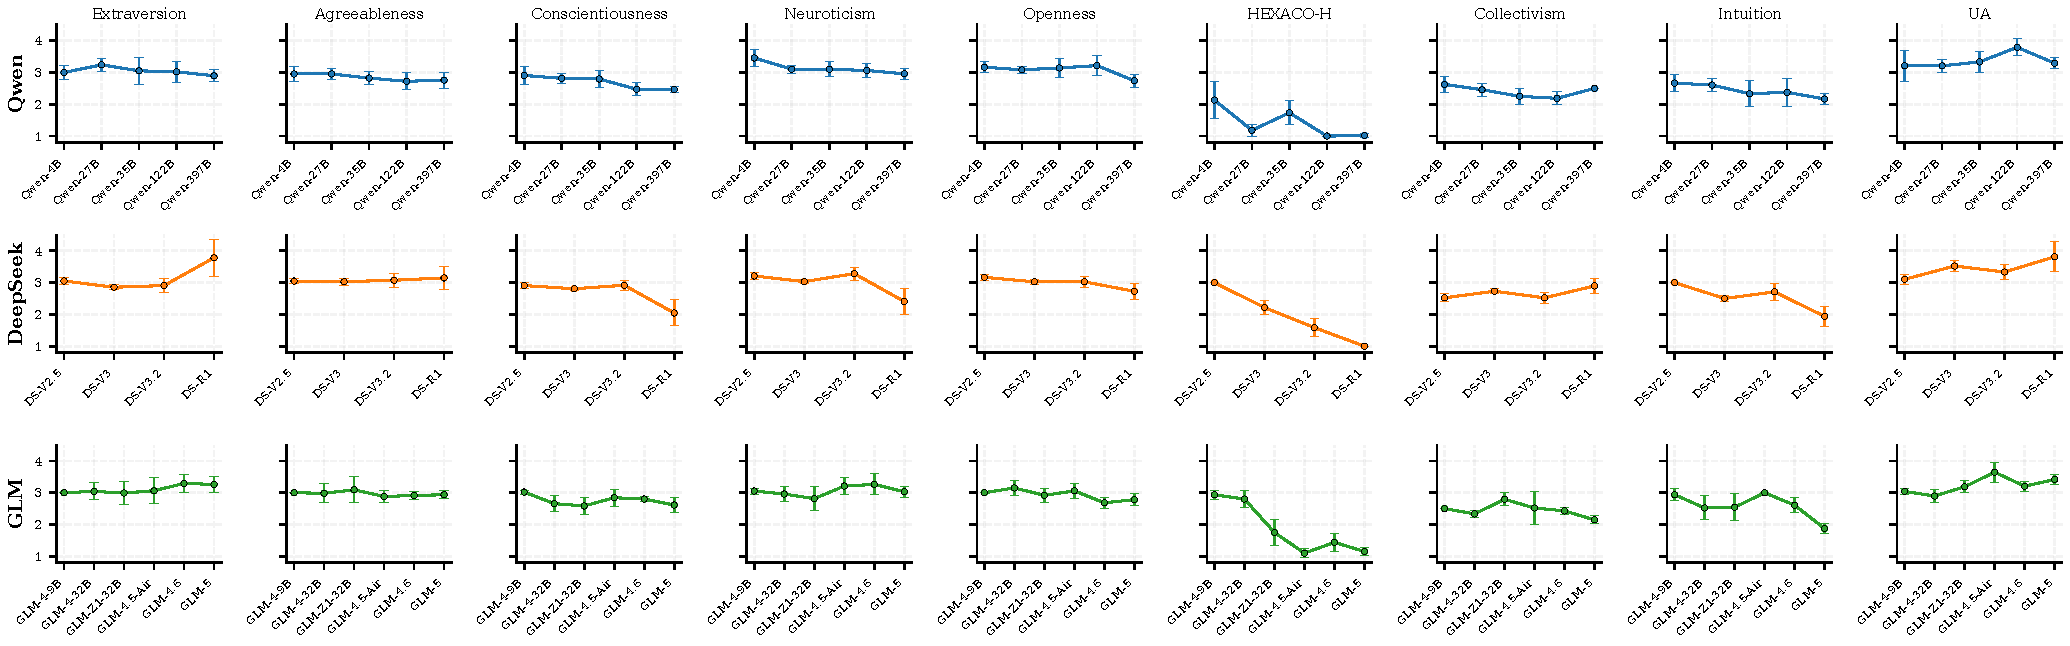
\includegraphics[width=0.95\textwidth]{figures/fig_study2_trajectories_combined.pdf}
    \caption{Within-family response style trajectories across model versions. Each row is one model family (Qwen, DeepSeek, GLM); each column is one dimension. Error bars show $\sd$ across seeds.}
    \label{fig:trajectories}
\end{figure*}

Qwen contributes 6 versions (4B to 397B), DeepSeek contributes 4 versions (V2.5 to R1), and GLM contributes 6 versions (GLM-4 to GLM-5).
Most dimensions show moderate variation across versions without clear monotonic trends.
Notable exceptions:
DeepSeek shows the steepest HEXACO-H collapse of any family, from V2.5 ($H = 3.00$) to V3.2 ($H = 1.68$), a drop of 1.32 points consistent with intensified safety alignment between versions.
GLM shows the largest within-family shift on Intuition (Cognitive Style), declining from 5.0 to 3.875 across versions.
These trajectories are descriptive (2--6 data points per family) and are included to motivate future controlled experiments with more data points per trajectory.

\end{document}
